\chapter{Funzioni in più variabili}
All'interno di questo capitolo si affronterà lo studio sistematico delle proprietà di funzioni in più variabili reali.\\
Nello specifico, si considereranno funzioni della forma: 
\begin{equation}
    f:\mathbb{R}^n \to \mathbb{R}^m
\end{equation}
con $m=1$, le cosiddette funzioni scalari, per poi passare al caso $m>1$, cioè le funzioni a valori vettoriali.
\section{Richiami di topologia in $\mathbb{R}^n$}
Per poter trattare lo studio di funzioni in più variabili occorre prima studiare la topologia dello spazio in cui si lavora.
In particolare, si può osservare che $\mathbb{R}^n$ è uno spazio vettoriale euclideo \textbf{normato}.
\begin{definition}
    Si dice che uno spazio $\mathbb{K}^n$ è \textbf{normato} se per ogni suo elemento $x=(x_1,\dots,x_n) \in \mathbb{K}^n$ la norma è ben definita. Nel caso di $\mathbb{R}^n$, si ha che:
    \begin{equation}
        |x|=\sqrt{\sum\limits_{i=1}^{n}{x_i^2}}
    \end{equation}
\end{definition}
Tramite la definizione di norma si può ottenere la definizione di \textbf{distanza}, grazie alla quale $\mathbb{R}^n$ può essere definito anche come spazio metrico.
\begin{definition} \label{Def: Distanza}
    Sia $X$ un insieme e sia $d:X \times X \to \left[0, +\infty \right)$ una funzione che ad ogni coppia $(x,y)$ di punti di $X$ associa un numero reale $d(x,y)\geq0$. Allora si dice che $d$ è una \textbf{distanza} o \textbf{metrica}su $X$ se sono verificate le seguenti condizioni:
    \begin{align}
        &d(x,y)=0 \ \iff x=y \qquad\forall\ x,y \in X \\
        &d(x,y)=d(y,x) \qquad \forall\ x,y \in X \\
        &d(x,y) \leq d(x,z) + d(z, y) \qquad \forall\ x,y,z \in X
    \end{align}
    In particolare in $\mathbb{R}^n$ si ha che:
    \begin{equation}
        d(x, y)=|x-y|
    \end{equation}
\end{definition}
\begin{definition}
    Sia $x_0$ un elemento di $\mathbb{R}^n$ fissato e sia $\delta>0$ un intero fissato. Si dice \textbf{intorno sferico} di $x_0$ di raggio $\delta$ la sfera aperta e non vuota di centro $x_0$ definita analiticamente come:
    \begin{equation}
        B_\delta(x_0)=\left\{x \in \mathbb{R}^n \ \mid \ d(x, x_0) < \delta \right\}
    \end{equation}
    \end{definition}
    \begin{oss}
        Si noti che con \textit{aperta} si intende dire che nell'intorno sferico non sono presenti elementi tali che $d(x, y)=\delta$.
    \end{oss}
    \begin{example}
        Un esempio di intorno sferico può essere la circonferenza in $\mathbb{R}^2$ di raggio $\delta=1$ centrata in $(x_0, y_0) \in \mathbb{R}^2$ definita come:
        \begin{equation*}
            B_1(x_0, y_0)= \{(x,y) \in \mathbb{R}^2 \ \mid \ \sqrt{(x-x_0)^2+(y-y_0)^2}< 1\}
        \end{equation*}
    \end{example}
\begin{definition}
    Siano $E \subseteq \mathbb{R}^n$ e $x_0 \in \mathbb{R}^n$. Allora $x_0$ è detto \textbf{punto interno} per $E$ se 
    \begin{equation}
        \exists\ \delta>0 \text{ tale che } B_\delta(x_0) \subseteq E 
    \end{equation}
    Si indica poi l'insieme dei punti interni di $E$ con $\mathring{E}$ oppure con int(E).
\end{definition}
\begin{definition}
    Siano $E \subseteq \mathbb{R}^n$ e $x_0 \in \mathbb{R}^n$. Allora $x_0$ è detto \textbf{punto esterno} per $E$ se 
    \begin{equation}
        \exists \ \delta>0 \text{ tale che } B_\delta(x_0) \subseteq E^\complement = \mathbb{R}^n \setminus E
    \end{equation}
    Si indica poi l'insieme dei punti esterni di $E$ con ext(E).
\end{definition}
\begin{definition}
    Siano $E \subseteq \mathbb{R}^n$ e $x_0 \in \mathbb{R}^n$. Allora $x_0$ è detto \textbf{punto di frontiera} per $E$ se 
    \begin{equation}
        \forall \ \delta>0 \text{ si ha che } B_\delta(x_0) \cap E \neq \emptyset \land B_\delta(x_0) \cap E^\complement \neq \emptyset 
    \end{equation}
    Si indica poi l'insieme dei punti di frontiera di $E$ con $\partial{E}$.
\end{definition}
\begin{definition}
    Siano $E \subseteq \mathbb{R}^n$ e $x_0 \in \mathbb{R}^n$. Allora $x_0$ è detto \textbf{punto di accumulazione} per $E$ se 
    \begin{equation}
        \forall \ \delta>0 \text{ si ha che } B_\delta(x_0) \cap \left(E \setminus \{x_0\}\right) \neq \emptyset
    \end{equation}
\end{definition}
\begin{definition}
    Siano $E \subseteq \mathbb{R}^n$ e $x_0 \in \mathbb{R}^n$. Allora $x_0$ è detto \textbf{punto isolato} se esso appartiene alla frontiera di $E$ ma non è di accumulazione.
\end{definition}
\begin{proposition}
    L'insieme dei punti interni, esterni e di frontiera di $E \in \mathbb{R}^n$ è una partizione di $\mathbb{R}^n$.
\end{proposition}
\begin{example}
    Sia $E$ così definito:
    \begin{equation*}
        E \subseteq \mathbb{R}^2 \mid E= B_1(0,0) \cup \{(x,y) \in \mathbb{R}^2\ \mid \ x>0, \ x^2+ y^2=1\} \cup \left\{\left(1,\tfrac{3}{2}\right)\right\}
    \end{equation*}
    \begin{minipage}{0.3\textwidth}
        \centering
        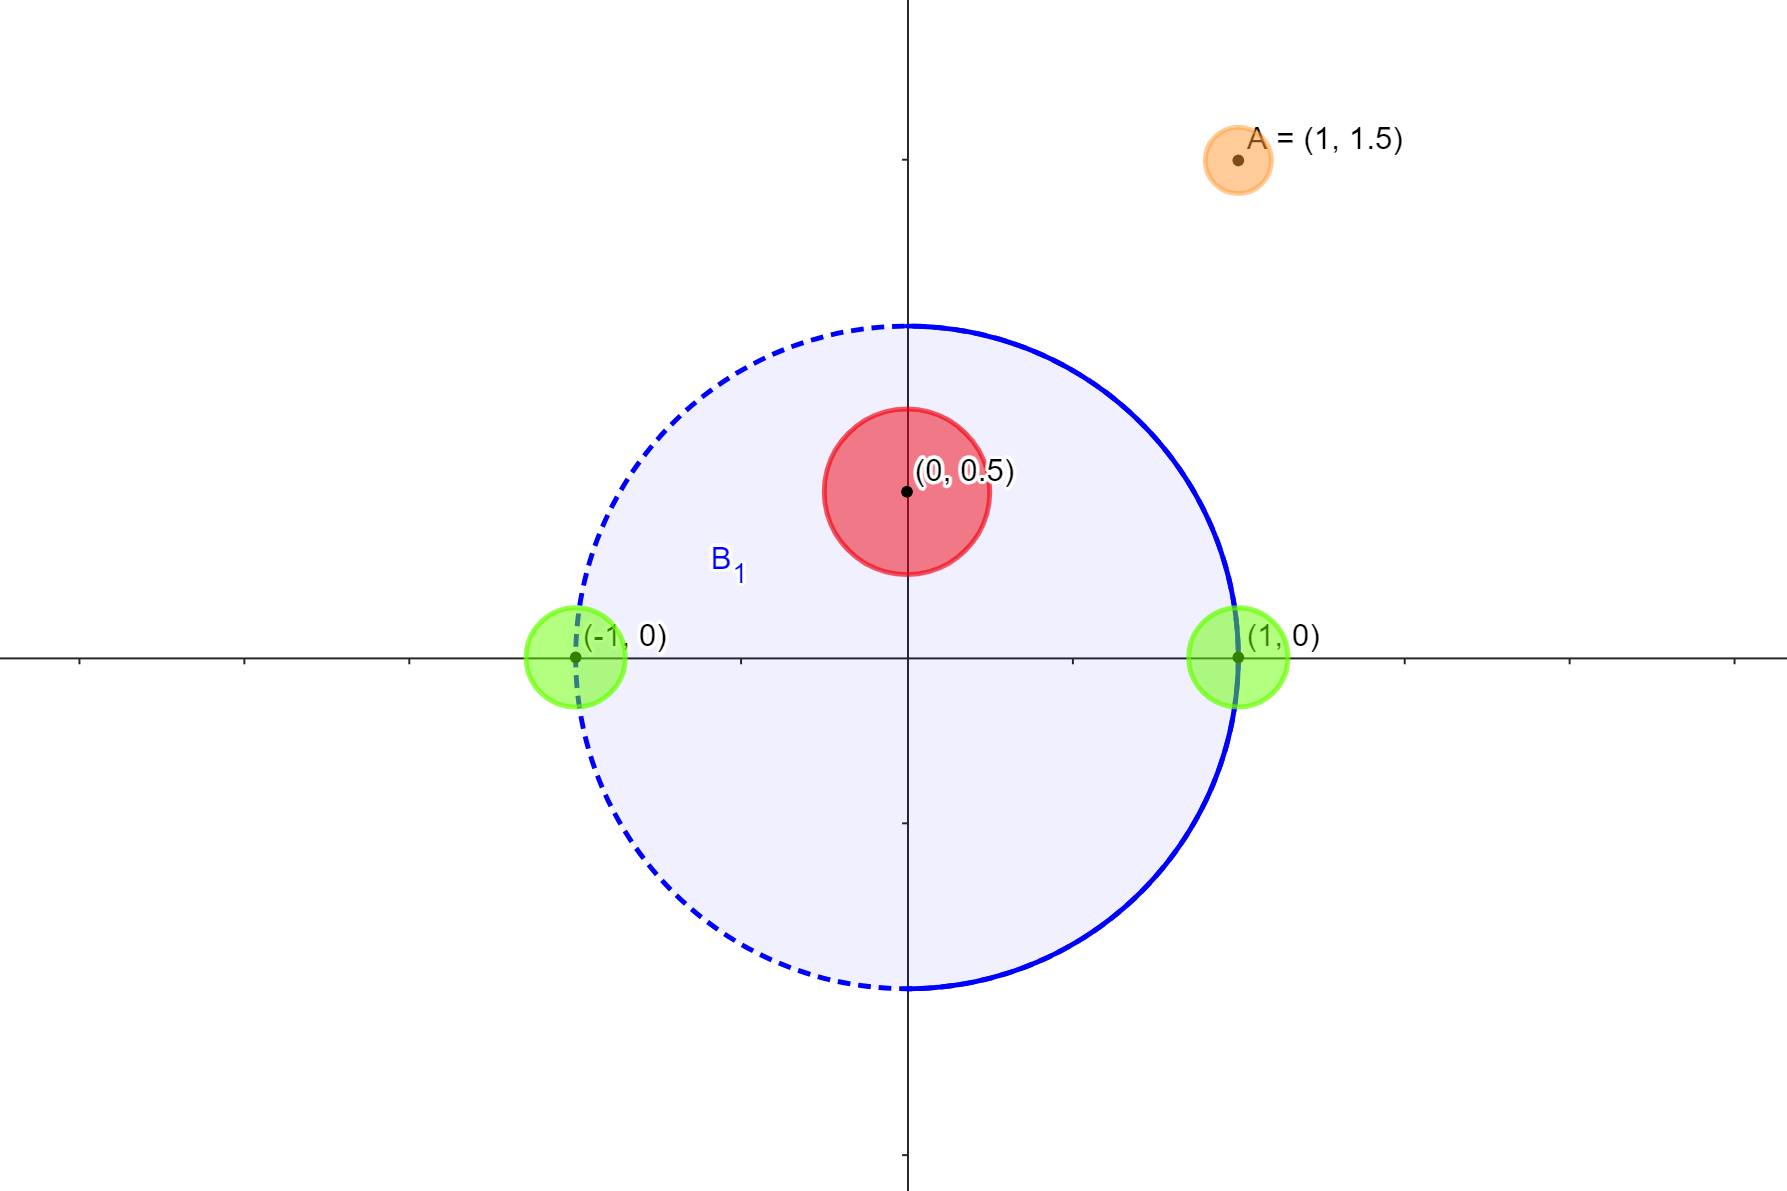
\includegraphics[width=\textwidth]{Capitoli/Capitolo2/Punti2.png}
    \end{minipage}
    \hfill
    \begin{minipage}{0.55\textwidth} 
        Si può dunque osservare che:
        \begin{itemize}
            \item $(0, \tfrac{1}{2})$ è \textit{interno}.
            \item $(1,0) $ è di \textit{frontiera} e di \textit{accumulazione}.
            \item $(-1,0) $ è di \textit{frontiera} e di \textit{accumulazione}.
            \item $\left(1, \tfrac{3}{2}\right) $ è di \textit{frontiera} e \textit{isolato}.
        \end{itemize}      
    \end{minipage}
\end{example}
\begin{definition}
    Un insieme $E \subseteq \mathbb{R}^n$ si dice \textbf{aperto} se
    \begin{equation}
        E=\mathring{E} \text{ oppure } E \cap \partial{E} = \emptyset
    \end{equation}
    ovvero se non ha punti esterni.
\end{definition}
\begin{definition} \label{Def: Insieme chiuso e chiusura}
    Si dice che un insieme $E \subseteq \mathbb{R}^n$ è \textbf{chiuso} se 
    \begin{equation}
        \partial{E} \subseteq E
    \end{equation}
    ovvero se $E^\complement$ è aperto.\\
    Si definisce poi \textbf{chiusura} di $E$ l'insieme
    \begin{equation}
        \overline{E} = E \cap \partial{E}
    \end{equation}
    Quindi un'altra definizione di insieme chiuso è:
    \begin{equation}
        E \text{ chiuso } \iff E=\overline{E}
    \end{equation}
\end{definition}
\begin{proposition}
    Un insieme $E$ è chiuso $\iff$ $E$ contiene tutti i suoi punti di accumulazione.
\end{proposition}
\begin{oss}
    $E=\{x_0\}$ con $x_0 \in \mathbb{R}^n$ fissato è chiuso e $E=\partial{E}$.
\end{oss}
\begin{oss}
    Dalla definizione, $\emptyset$ e $\mathbb{R}^n$ sono entrambi contemporaneamente aperti e chiusi e sono gli unici sottoinsiemi di $\mathbb{R}^n$ con tali proprietà.
\end{oss}
\begin{definition}
    Sia $E \subseteq \mathbb{R}^n$, $E$ si dice \textbf{limitato} se
    \begin{equation}
        \exists\ R>0 \text{ tale che } E \subseteq B_R(0)
    \end{equation}
    Altrimenti esso è detto \textbf{illimitato}.
\end{definition}
\begin{definition}
    Un insieme aperto $A\subseteq \mathbb{R}^n$ si dice \textbf{connesso} se non esistono due aperti $A_1, \ A_2$ non triviali (cioè diversi da $\emptyset,\ \mathbb{R}^n,\ A$) e disgiunti tali che
    \begin{equation}
        A=A_1 \cup A_2
    \end{equation}
\end{definition}
\begin{definition}
    Sia $E \subseteq \mathbb{R}^n$. Allora $E$ si dice \textbf{connesso per archi} se per ogni $(x,y) \in E$ esiste una curva parametrica $\varphi:[0,1] \to E$ tale che
    \begin{equation}
        \varphi(0)=x \land \varphi(1)=y
    \end{equation}
\end{definition}
\begin{definition}
   $E \subseteq \mathbb{R}^n$ si dice \textbf{dominio} (\textbf{connesso}) se è la chiusura di un aperto (connesso).
\end{definition}
\begin{definition}
    Un insieme $E \subseteq \mathbb{R}^n$ si dice \textbf{convesso} se, definito $[x,y]$ il segmento di estremi $x,\ y$ si ha che
    \begin{equation}
        [x,y] \subseteq E
    \end{equation}
    \end{definition}
    \begin{oss}
        Un insieme convesso è per definizione connesso per archi.
    \end{oss}
\begin{definition}
    Un insieme $E \subseteq \mathbb{R}^n$ si dice \textbf{stellato} rispetto ad un punto $x_0$ di E se per ogni $x$ di $E$ si ha che
    \begin{equation}
        [x_0, x] \subseteq E
    \end{equation}
\end{definition}

%%  DEFINIZIONI SEQUENZIALI


\section{Definizioni sequenziali}
\begin{definition}
    Si dice \textbf{successione in $\mathbb{R}^n$} una funzione da $\mathbb{N}$ a valori in $\mathbb{R}^n$.
    \begin{equation}
        (x_k)_{k \in \mathbb{N}} = ((x_k)_1, \dots, (x_k)_n)  
    \end{equation}
    con $k \in \mathbb{N}$ indice intero della successione.
\end{definition}
\begin{definition}
    Sia $(x_k)_k$ una successione in $\mathbb{R}^n$. Si dice che $x_k$ \textbf{converge} a $\ell$, cioè
    \begin{equation}
        x_k \to \ell=(\ell_1, \dots, \ell_n) \in \mathbb{R}^n
    \end{equation}
    se la loro distanza converge a zero. Poiché 
    \begin{equation}
        d(x_k, \ell)=|x_k-\ell|=\sqrt{[(x_k)_1-\ell_1]^2+\dots+[(x_k)_n-\ell_n]^2}
    \end{equation}
    la successione converge se ogni sua componente converge a ciascuna componente di $\ell$, quindi
    \begin{equation}
        (x_k)_k \overset{k\to+\infty}{\to} \ell \iff (x_k)_i \overset{k\to+\infty}{\to} \ell_i \ \forall i
    \end{equation}
\end{definition}
\begin{definition}
    Sia $(x_k)_k$ una successione di vettori di $\mathbb{R}^n$. Si dice che $x_k$ \textbf{diverge} se
    \begin{equation}
        |x_k| \overset{k\to+\infty}{\to} \infty
    \end{equation}
    \end{definition}
    \begin{oss}
        Si osservi che è sufficiente che la norma di una sola componente di $x_k$ diverga affinché la successione sia divergente.
        \begin{example}
            Presa come successione $x_k=\left(\frac{1}{k}, k\right)$, poiché la sua seconda componente è divergente per $k \to \infty$, anche la successione lo è.
        \end{example}
    \end{oss}
\begin{definition} \label{Def: Punto di accumulazione}
    Sia $E \subseteq \mathbb{R}^n$ e sia $x_0 \in \mathbb{R}^n$. Si dice che $x_0$ è \textbf{punto di accumulazione} per $E$ se
    \begin{equation}
        \exists\ (x_k)_k \text{ con } x_k\neq x_0 \in E \ \forall \ k \text{ tale che } x_k \to x_0
    \end{equation}
\end{definition}
\begin{definition}
    Sia $K \subseteq \mathbb{R}^n$. Si dice che $K$ è un insieme \textbf{compatto} se da ogni successione $(x_k)_k$ è possibile estrarre una sottosuccessione convergente ad un punto di $K$
\end{definition}
\begin{theorem}[Heine-Borel] \label{Teo: Heine Borel}
    Un insieme $K$ è compatto se e solo se è chiuso e limitato.
\end{theorem}
    \begin{oss}
        Un insieme $C \subseteq \mathbb{R}^n$ è chiuso se e solo se per ogni successione di elementi in $C$ convergente si ha che il limite di tale successione è contenuto in $C$.
    \end{oss}

%%  INTRODUZIONE FUNZIONI IN PIU VARIABILI

\section{Introduzione alle funzioni in più variabili}
Come già anticipato, da questo momento in avanti si studieranno prima le funzioni scalari e poi quelle a valori vettoriali.
Si cominci prima da alcune definizioni di carattere generale. 
\begin{definition}
    Si dice \textbf{dominio} di una funzione $f$ di $n$ variabili il più grande sottoinsieme di $\mathbb{R}^n$ su cui $f$ è definita. Esso viene indicato con $\text{dom}(f)$.
\end{definition}
\begin{definition}
    Sia $f: \Omega \subseteq \mathbb{R}^n \to \mathbb{R}$. Si dice \textbf{grafico} di $f$ il sottoinsieme di $\mathbb{R}^{n+1}$
    \begin{equation}
        G(f)= \left\{(x_1, \dots, x_n, x_{n+1}) \in \Omega \times \mathbb{R} \mid x_{n+1}=f(x)\right\}
    \end{equation}
\end{definition}
\begin{definition}
    Sia $f:\Omega \subseteq \mathbb{R}^n \to \mathbb{R}$ e sia $l \in \mathbb{R}$. Si dice \textbf{superficie di livello} o \textbf{ipersuperficie} $l$ per $f$ il sottoinsieme
    \begin{equation}
        L_l=\left\{x \in \Omega \mid f(x)=l\right\}=f^{-1}(l)
    \end{equation}
\end{definition}

%%   LIMITI
\section{Limiti}
\begin{definition}[Limiti al finito] \label{Def: Limiti al finito}
    Sia $f:\Omega \subseteq \mathbb{R}^n \to \mathbb{R}$ e sia $x_0$ un punto di accumulazione per l'insieme $\Omega$.\\
    Si dice che $f$ \textbf{converge} a $\ell \in \mathbb{R}$ per $x \to x_0$ e si scrive
    \begin{equation}
        \lim_{x \to x_0}{f(x)}=\ell
    \end{equation} 
    se
    \begin{equation}
        \forall \varepsilon>0 \ \exists\delta=\delta_\varepsilon>0\ \text{tale che, se}\ 
                x \in B_\delta(x_0) \setminus \left\{x_0\right\}\ \cap\ \Omega
            \text{ allora}\ |f(x)-\ell|<\varepsilon
    \end{equation}
    Analogamente, si dice che $f$ \textbf{diverge} per $x \to x_0$ con $x \in \Omega$ e si scrive
    \begin{equation}
        \lim_{x \to x_0}{f(x)}=\underset{-\infty}{+\infty}
    \end{equation}
    se 
    \begin{equation}
        \forall M>0 \ \exists\delta=\delta_M>0\ \text{tale che, se}\ 
        x \in B_\delta(x_0) \setminus \left\{x_0\right\}\ \cap\ \Omega
            \text{ allora}\ \underset{f(x)<-M}{f(x)>M}
    \end{equation}
\end{definition}
\begin{definition}
    Sia $f:\Omega \subseteq \mathbb{R}^n$ con $x_0$ punto di accumulazione. Si dice che 
    \begin{equation}
        \lim_{x \to x_0}{f(x)}=\ell
    \end{equation}
    se per ogni successione di punti di $\Omega$ $(x_k)_k$ diversi da $x_0$ tali che
    \begin{equation}
        f(x_k)\to \ell
    \end{equation}
    \end{definition}
    \begin{oss}
        La definizione è analoga per i casi in cui $\ell$ sia infinito.
    \end{oss}
    \begin{oss}
        Stando alla definizione \ref{Def: Punto di accumulazione}, l'ipotesi di di $x_0$ punto di accumulazione garantisce l'esistenza di almeno una successione convergente.
    \end{oss}
\begin{definition}[Limiti all'infinito] \label{Def: Limiti all'infinito}
    Sia $f:\Omega \to \mathbb{R}$. Allora, 
    \begin{equation}
        \lim_{x \to \infty}{f(x)}=\ell
    \end{equation}
    se
    \begin{equation}
        \forall \varepsilon > 0 \ \exists k=k_\varepsilon>0 \ \text{tale che, se}\ |x|>k_\varepsilon,\ \text{allora}\ |f(x)-\ell|<\varepsilon
    \end{equation}
    Analogamente,
    \begin{equation}
        \lim_{x \to \infty}{f(x)}=\underset{-\infty}{+\infty}
    \end{equation}
    se 
    \begin{equation}
        \forall M>0 \exists k=k_M>0 \ \text{tale che, se}\ |x|>k_M\ \text{allora}\ \underset{f(x)<-M}{f(x)>M}
    \end{equation}
\end{definition}
\subsection{Metodi per la risoluzione di limiti}
Il discorso che segue parte dal caso specifico di funzioni in due variabili ma può essere generalizzato con le dovute accortezze al caso di funzioni in $n$ variabili.\\
Si parta dallo specificare che anche per i limiti di funzioni multivariabile è possibile utilizzare le approssimazioni asintotiche.\\
Stando alla definizione di limite, esso non deve dipendere da come ci si avvicina a $x_0$. In prima istanza occorre allora scegliere uno degli innumerevoli metodi per farlo, noti come restrizioni. Tramite questi, è possibile trovare un candidato limite la cui esistenza deve essere verificata in uno dei modi che verranno illustrati.\\
Si può osservare che, se la funzione tende ad un limite $\ell$, allora esso è unico e valgono i teoremi delle funzioni in una variabile su somme, prodotti e quozienti di limiti; inoltre, se il limite esiste, $f$ tende (e deve tendere) a $\ell$ lungo ogni sua possibile restrizione. Viceversa, se esistono almeno due restrizioni il cui limite sia differente, il limite non esiste.\\
L'approccio per trovare il candidato limite ammette
\begin{itemize}
    \item Restrizioni lungo grafici di funzioni di $x$ o $y$ passanti per $(x_0, y_0)$ e appartenenti al dominio di $f$. In tal caso le funzioni possono essere $y= \varphi(x)$ o $x=\psi(y)$ e si avrà
    \begin{equation}
    \lim_{x \to x_0} f(x, \varphi(x)) \text{ o } \lim_{y \to y_0}{f(\psi(y), y)}
    \end{equation}
    \item Restrizioni lungo successioni $(x_n, y_n) \to (x_0, y_0)$ e in tal caso si calcola
    \begin{equation}
        \lim_{n \to +\infty}{f(x_n,y_n)}
    \end{equation}
    \item Restrizioni lungo curve parametriche $(x(t), y(t)): I \to \mathbb{R}^2$ passanti per $(x_0, y_0)$. In tal caso si calcola
    \begin{equation}
        \lim_{t \to t_0}{f(x(t), y(t))}
    \end{equation}
\end{itemize}
Si mostrino di seguito alcuni modi per provare l'esistenza del limite.
\subsubsection{Definizione}
Per conseguire il risultato prefissato occorre maggiorare o minorare la funzione in maniera tale da trovare un $\delta_\varepsilon$ per cui la definizione di limite sia verificata.
\begin{example}
    Si mostri il procedimento sul seguente limite.
    \begin{equation*}
        \lim_{(x,y) \to (0,0)}x
    \end{equation*}
    Attraverso la restrizione $(0,y)$ si può osservare che il candidato limite è $0$. Ora occorre provare che ciò sia vero.
    Dunque bisogna capire se sia possibile trovare un $\delta$ dipendente da $\varepsilon$ per cui sotto l'ipotesi
    \begin{equation*}
        \begin{cases}
            0<|(x,y)-(0,0)|<\delta\\
            (x,y) \in \text{dom}f
        \end{cases}
    \end{equation*}
    si abbia $|x-0|<\varepsilon$.\\
    Fissato $\varepsilon$ e sapendo che $|x|=\sqrt{x^2+y^2}<\delta$, serve provare che $|x|<\varepsilon$. Ciò è vero scegliendo $\delta<\varepsilon$.\\
    Al contrario, preso qualsiasi altro valore di $\ell$ la definizione non è verificata, come ci si aspetta.
\end{example}
\subsubsection{Confronto}
Così come avveniva nelle funzioni a una variabile, è possibile verificare un candidato limite maggiorandolo e minorandolo con funzioni convergenti al medesimo candidato limite, applicando, cioè, il metodo del confronto.
\begin{example}
    Si calcoli il limite seguente.
    \begin{equation*}
        \lim_{(x,y) \to (0,0)}{\frac{xy}{\sqrt{x^2+y^2}}}
    \end{equation*}
    Tramite la restrizione su uno dei due assi si ottiene $0$ come candidato limite.
    Siccome vale la disuguaglianza di Young, che afferma che 
    \begin{equation*}
        xy \leq \frac{x^2+y^2}{2}
    \end{equation*}
    si può verificare che
    \begin{equation*}
        0 \leq \left|\frac{xy}{\sqrt{x^2+y^2}}\right| \leq \frac{\sqrt{x^2+y^2}}{2}
    \end{equation*}
    con gli estremi convergenti a $0$. Pertanto, il limite esiste ed è $0$.
\end{example}
\subsubsection{Coordinate polari}
Dal momento che per provare la definizione di limite si deve controllare una distanza, può essere utile passare alle coordinate polari centrate nel punto $(x_0, y_0)$, ottenendo
\begin{equation}
    \begin{cases}
        x=x_0+ \varrho \cos(\theta)\\
        y=y_0+ \varrho \sin(\theta)
    \end{cases}
\end{equation}
Così facendo, fissato $\theta$ e fatto convergere $\varrho \to 0^+$, il limite diventa
\begin{equation}
    \lim_{\varrho\to 0}{f(x_0+\varrho\cos(\theta), y_0+\varrho\sin(\theta))}=\ell
\end{equation}
Si consegue così una condizione necessaria per l'esistenza del limite. È tuttavia possibile estendere tale affermazione ad una condizione necessaria e sufficiente ricercando un criterio tale da rendere il risultato univocamente determinato da $\varrho$ (e valido così $\forall\ \theta$).
\begin{theorem} \label{Teo: Condizione necessaria e sufficiente per un limite}
    Sia $f(x,y): E \subseteq \mathbb{R}^2 \to \mathbb{R}$ e sia $(x_0, y_0)$ punto di accumulazione per $\text{dom}f$ e sia $\ell \in \mathbb{R}$. Allora esiste
    \begin{equation}
        \lim_{(x,y)\to(x_0, y_0)}f(x,y)=\ell
    \end{equation}
    se e solo se esistono $r>0$ e $g:(0, r) \to \mathbb{R}$ tali che
    \begin{equation}
        \lim_{\varrho \to 0^+}{g(\varrho)=0}
    \end{equation}
    e, per ogni $\theta \in [0, 2\pi],\ \varrho\in (0, r)$ si ha che 
    \begin{equation}
        \left|f(x_0+\varrho\cos(\theta), y_0+\varrho\sin(\theta))-\ell \right|\leq g(\varrho)
    \end{equation}
\end{theorem}
\begin{example}
    Si calcoli nuovamente questo limite.
    \begin{equation*}
        \lim_{(x, y) \to (0,0)}{\frac{xy}{\sqrt{x^2+y^2}}}
    \end{equation*}
    Come prima, il candidato limite è $0$.\\
    Applicando un cambio di coordinate si ha che
    \begin{equation*}
        \begin{cases}
            x=\varrho\cos(\theta)\\
            y=\varrho\sin(\theta)
        \end{cases}
    \end{equation*}
    e, dunque, $f$ diviene
    \begin{equation*}
        f(\varrho\cos(\theta),\varrho\sin(\theta))=\frac{\varrho^2\cos(\theta)\sin(\theta)}{\varrho}=\varrho\cos(\theta)\sin(\theta)
    \end{equation*}
    Di conseguenza,
    \begin{equation*}
        |f(\varrho\cos(\theta),\varrho\sin(\theta))- \ell|=\varrho\cos(\theta)\sin(\theta) \leq \varrho = g(\varrho)
    \end{equation*}
    Pertanto, il limite esiste ed è verificato.
\end{example}
\begin{example}
    Si fornisca ora un esempio di limite non definito.
    \begin{equation*}
        \lim_{(x,y) \to (0,0)}{\frac{xy}{x^2+y^2}}
    \end{equation*}
    Per dimostrare l'inesistenza di $\ell$ si può procedere innanzitutto sfruttando le restrizioni. Infatti, se prendendo come cammini gli assi, il candidato limite è $0$, prendendo una retta generica della forma $y=mx$ tale risultato non è comprovato.
    \begin{equation*}
        \lim_{(x, mx) \to (0,0)}{\frac{x^2m}{x^2+x^2m^2}}=\lim_{(x, mx) \to (0,0)}{\frac{m}{m^2+1}} \neq 0
    \end{equation*}
    In alternativa, si può verificare ciò con il teorema \ref{Teo: Condizione necessaria e sufficiente per un limite}. In coordinate polari il limite diviene
    \begin{equation*}
        \lim_{\varrho \to 0^+}{\left|\frac{\varrho^2\cos(\theta)\sin(\theta)}{\varrho^2}\right|}=\lim_{\varrho \to 0^+}{\left|\cos(\theta)\sin(\theta)\right|} < \frac{1}{2}=g(\varrho)
    \end{equation*}
    Ma $g(\varrho)$ non tende a $0$ per $\varrho \to 0^+$ quindi, il limite si riconferma indefinito.
\end{example}
\subsection{Continuità}
Si sfruttino ora le nozioni apprese sui limiti per definire la continuità di una funzione.
\begin{definition} \label{Def: Continuità}
    Sia $f: E \subseteq \mathbb{R}^n \to \mathbb{R}$ e sia $x_0 \in \mathbb{R}^n$. Se $x_0$ è un punto isolato di E, la funzione si dice \textbf{continua} in $x_0$ per convenzione. Se $x_0$ è di accumulazione per E, f è \textbf{continua} in $x_0$ se è definita in tale punto e
    \begin{equation} \label{Eq: Continuità}
        \lim_{x \to x_0} f(x)= f(x_0)
    \end{equation}
    ovvero, in termini di $\varepsilon$ e $\delta$, se
    \begin{equation}
        \forall \varepsilon > 0 \  \exists \delta>0 \text{ tale che se } x \in B_\delta(x_0) \cap E, \ |f(x)-f(x_0)|< \varepsilon
    \end{equation}
    \end{definition}
    \begin{oss}
        Se f non è definita in $x_0$ ma esiste il limite $\ell$ di $f(x)$ per $x \to x_0$, è possibile definire il \textbf{prolungamento di continuità} per $f$ in $x_0$ come:
        \begin{equation}
            g(x) = \begin{cases}
                f(x) \text{ se } x \neq x_0, x \in \text{dom}f\\
                \ell \text { se } x=x_0
            \end{cases}
        \end{equation}
    \end{oss}
    \begin{oss}
        Rientrano tra le funzioni continue somme, prodotti, quozienti (ben definiti) di polinomi
    \end{oss}
\vspace*{\baselineskip}
Si noti che anche per funzioni in più variabili continue vale un analogo del teorema di \textbf{permanenza del segno}, che afferma che, se $f$ è definita in $B_\delta(x_0)$ ed è continua in $x_0$ con $f(x_0) \gtrless 0$, allora esiste $B_\delta'(x_0)$ con $\delta' \leq \delta$ su cui il segno viene mantenuto.
\begin{definition}
Sia $f:X \subseteq \mathbb{R}^n \to \mathbb{R}$. Si dice che $x_0 \in X$ è \textbf{punto di massimo assoluto} (forte) per $f$ in $X$ se
\begin{equation}
    \begin{aligned}
        f(x) \leq f(x_0) \ \forall x  \in X \\
        (f(x) < f(x_0) \ \forall x  \in X)
    \end{aligned}
\end{equation}
In tal caso, $f(x_0)$ è detto \textbf{valore massimo} di $f$ su $X$.\\
In maniera del tutto analoga, data $f:X \subseteq \mathbb{R}^n \to \mathbb{R}$, si dice che $x_0 \in X$ è \textbf{punto di minimo assoluto} (forte) per $f$ in $X$ se
\begin{equation}
    \begin{aligned}
        f(x) \geq f(x_0) \ \forall x \in X\\
        (f(x)>f(x_0) \ \forall x \in X)
    \end{aligned}
\end{equation}
In tal caso, $f(x_0)$ è detto \textbf{valore minimo} di $f$ su $X$
\end{definition}
\begin{theorem}[Weierstrass] \label{Teo: Weierstrass}
    Sia $K \subseteq \mathbb{R}^n$ compatto e sia $f: K \to \mathbb{R}$ continua su $K$. Allora, esistono $x_m, x_M$ tali che
    \begin{equation}
    \min_{x \in K}{f(x)}= f(x_m) \leq f(x) \leq f(x_M) = \max_{x \in K}{f(x)}    
    \end{equation}
\end{theorem}
    \begin{oss}
        Una possibile notazione di min e max è $ \min\limits_{K}{f}$ e $\max\limits_{K}{f}$.
    \end{oss}
\begin{theorem}[Valori intermedi] \label{Teo: Valori intermedi}
    Sia $D \subseteq \mathbb{R}^n$ un dominio connesso (cioè la chiusura di un aperto connesso) e limitato. Allora $D$ è compatto per il teorema \ref{Teo: Heine Borel}.
    Sia poi $f:D \to \mathbb{R}$ continua su $D$. Allora $f$ assume su $D$ tutti i valori compresi tra $\min\limits_{D}{f}$ e $\max\limits_{D}{f}$ cioè
    \begin{equation}
        f(D)=\left[ \min_{D}{f}, \max_{D}{f}\right]
    \end{equation}
\end{theorem}
    \begin{oss}
        Se $D$ non è limitato, si ragiona su $\sup_{D}{f}$ e $\inf_{D}{f}$ anziché in termini di massimo e minimo.
    \end{oss}
\begin{corollary}[Teorema degli zeri] \label{Teo: Teorema degli zeri}
    Sia $f$ tale da rispettare le ipotesi del teorema \ref{Teo: Valori intermedi}. Siano poi $x_0, x_1 \in D$ tali che 
    \begin{equation}
        f(x_0)f(x_1) < 0
    \end{equation}
    allora, esiste $x^* \in D$ tale che $f(x^*)=0$.
\end{corollary}
\begin{definition} \label{Def: Uniforme continuità}
    Sia $f:E \subseteq \mathbb{R}^n \to \mathbb{R}$. Allora $f$ si dice \textbf{uniformemente continua} se
    \begin{equation}
        \forall \varepsilon >0 \ \exists \delta=\delta_\varepsilon\ \text{tale che}\ \forall x, y \in E\ \text{tali che}\ |x-y|<\delta\ \text{si ha che}\ |f(x)-f(y)| < \varepsilon
    \end{equation}
\end{definition}
\begin{theorem}[Heine Cantor] \label{Teo: Heine Cantor}
    Sia $f: K \subseteq \mathbb{R}^n \to \mathbb{R}$ continua con $K$ compatto. Allora $f$ è uniformemente continua su $K$.
\end{theorem}
Il teorema appena enunciato offre un metodo per verificare l'uniforme continuità su un compatto. Tuttavia, la definizione si applica su insiemi generici. Un metodo per verificare tale proprietà su insiemi non compatti è sfruttare la nozione di \textbf{lipschitzianità}.
\begin{definition} \label{Def: Funzione lipschitziana}
    Sia $f:E \subseteq \mathbb{R}^n \to \mathbb{R}$. Si dice che $f$ è \textbf{lipschitziana} su $E$ con costante di Lipschitz $L>0$ se
    \begin{equation}
        \forall\ x,y \in E\ \text{si ha che}\ |f(x)-f(y)| \leq L|x-y|
    \end{equation}
\end{definition}
\begin{proposition}
    Le funzioni lipschitziane su $E$ sono uniformemente continue.
\end{proposition}
    \begin{proof}
        Si applichi ad una funzione lipschitziana la definizione di uniforme continuità con 
        \begin{equation}
            \delta= \frac{\varepsilon}{L}
        \end{equation}
    \end{proof}
Se il discorso sulla continuità dovesse riguardare una funzione a valori vettoriali $f: \mathbb{R}^n \to \mathbb{R}^m$ con $m>1$ anziché scalari, le definizioni di limite e continuità rimangono valide a patto che le condizioni siano verificate componente per componente, cioè
\begin{equation}
    \lim_{x \to x_0}{f(x)}=\ell \in \mathbb{R}^m \iff \lim_{x \to x_0}{f_i(x)}=\ell_i\ \forall i=1, \dots, m
\end{equation}
\section{Derivate direzionali}
Si passi ora alla trattazione del calcolo di derivate per funzioni multivariabile. Per fare ciò occorre prima definire cosa sia una \textit{direzione}.
\begin{definition} \label{Def: Direzione}
    Si dice \textbf{direzione} un vettore $v \in \mathbb{R}^n$ tale che abbia norma unitaria. 
\end{definition}
Fatto ciò, si può iniziare a parlare effettivamente di derivate direzionali, ovvero dello studio della derivata di una funzione in più variabili lungo una determinata direzione.
\begin{definition}
    Sia $f: A \subseteq \mathbb{R}^n \to \mathbb{R}$ e sia $x_0 \in A$. Sia poi $v \in \mathbb{R}^n$ una direzione fissata.
    Si dice allora che $f$ è \textbf{derivabile} in $x_0$ lungo la direzione $v$ se esiste \textit{finito}
    \begin{equation}
        \lim_{t \to 0}{\frac{f(x_0+tv)-f(x_0)}{t}}= \ell
    \end{equation}
    che viene detto \textbf{derivata direzionale} di $f$ in $x_0$ lungo la direzione $v$ e viene annotato con 
    \begin{equation}
        \frac{\partial{f}}{\partial{v}}(x_0)
    \end{equation}
    \end{definition}
\begin{oss}
    È possibile mostrare l'equivalenza di questa definizione con quella delle funzioni in una variabile. Infatti, definita una generica
    \begin{equation}
        g(t)=f(x_0+tv)
    \end{equation}
    si ha che 
    \begin{equation}
        \frac{\partial{f}}{\partial{v}}(x_0) = \lim_{t \to 0}{\frac{f(x_0+tv)-f(x_0)}{t}} = \lim_{t \to 0}{\frac{g(t+0)-g(0)}{t}}=g'(0)
    \end{equation}
\end{oss}
\subsection{Derivate parziali}
Poiché esistono infinite direzioni, esistono altrettante derivate direzionali. Tra queste, dunque, occorre evidenziare $n$ direzioni privilegiate, ovvero i versori della base canonica $\mathcal{C}=\left\{e_1,\dots, e_n\right\}$. Lungo tali direzioni si hanno quindi le \textit{derivate parziali}.
\begin{definition} \label{Def: Derivate parziali}
    Si dicono \textbf{derivate parziali} le $n$ derivate in $x_0$ lungo un versore della base canonica e le si indica con
    \begin{equation}
        \frac{\partial{f}}{\partial{x_i}}
    \end{equation}
    dove con $x_i$ si mette in evidenza il fatto che la direzione sia privilegiata.
\end{definition}
La definizione di derivata parziale è dunque un caso particolare della derivata direzionale. La definizione di quest'ultima può essere rimodellata sulla prima così:
\begin{equation}
    \frac{\partial{f}}{\partial{x_i}}=\lim_{t \to 0}{\frac{f(x_0^1, \dots, x_0^i+t, \dots, x_0^n)-f(x_0^1, \dots, x_0^i, \dots, x_0^n)}{t}}
\end{equation}
Definite le direzioni privilegiate e le derivate parziali, si può ora formalizzare il concetto di derivabilità in un punto.
\begin{definition} \label{Def: Derivabilità}
    Sia $f:A \subseteq \mathbb{R}^n \to \mathbb{R}$ con $A$ aperto e sia $x_0 \in A$. Si dice che $f$ è \textbf{derivabile in $x_0$} se esistono finite le $n$ derivate parziali
    \begin{equation}
        \frac{\partial{f}}{\partial{x_i}}(x_0)
    \end{equation}
In tal caso si può definire un vettore di derivate in $x_0$. Tale vettore è detto \textbf{gradiente} e viene indicato con
\begin{equation}
    \nabla f(x_0) := \left(\frac{\partial{f}}{\partial{x_1}}(x_0), \dots, \frac{\partial{f}}{\partial{x_i}}(x_0), \dots, \frac{\partial{f}}{\partial{x_n}}(x_0)\right)\ \text{con}\ i \in [0,n]
\end{equation}
\end{definition}
Spesso il calcolo di una derivata parziale si riduce all'applicazione degli stessi metodi di differenziazione propri del calcolo differenziale di funzioni in una variabile con l'accortezza di considerare le altre variabili come costanti. Tuttavia non sempre è possibile farlo e occorre derivare tramite la definizione. Si mostrino alcuni esempi.
\begin{example}
    Sia $f(x, y)=xe^y$ e si voglia calcolare le due derivate parziali nel punto $(1,0)$.
    In generale le derivate parziali sono:
    \begin{equation*}
        \begin{aligned}
            \frac{\partial{f}}{\partial{x}}(x_0,y_0)=e^y \\
            \frac{\partial{f}}{\partial{x}}(x_0,y_0)=xe^y
        \end{aligned}
    \end{equation*}
    Quindi in $(1,0)$ si ha $\nabla f((1,0))=(1,1)$.
\end{example}
\begin{example}
    Sia $f(x,y)= yx^{\tfrac{2}{3}}$ e $(x_0, y_0)=(0,0)$.
    Allora,
    \begin{equation*}
        \frac{\partial{f}}{\partial{x}}(x_0,y_0)= \frac{2}{3}yx^{-\tfrac{1}{3}} \Big|_{(0,0)}
    \end{equation*}
    Tuttavia, la funzione non è di classe $C^1$ quindi bisogna usare la definizione.
    \begin{equation*}
        \frac{\partial{f}}{\partial{x}}(0,0)=\lim_{t \to 0}{\frac{f(t,0)-f(0,0)}{t}}=\lim_{t \to 0}{\frac{0-0}{t}}=0
    \end{equation*}
\end{example}
\begin{example}
    Sia $f(x,y)$ definita a tratti come segue
    \begin{equation*}
        f(x,y)= \begin{cases}
            \frac{xy^2}{x^2+y^4}\ &\text{se}\ (x,y)\neq (0,0)\\
            0\ &\text{se}\ (x,y)=(0,0)
        \end{cases}
    \end{equation*}
   e se ne calcolino le derivate direzionali in $(0,0)$.\\
   Non essendo la funzione continua, bisogna utilizzare la definizione.
   Si scelga allora come direzione un generico $v=(\cos(\alpha), \sin(\alpha))$.
   Quindi
   \begin{equation*}
    \begin{aligned}
        \frac{\partial{f}}{\partial{v}}(0,0)&=\lim_{t \to 0}{\frac{f((0,0)+t(\cos(\alpha), \sin(\alpha)))-f(0,0)}{t}}=\\
        &=\lim_{t \to 0}{\frac{f(t\cos(\alpha), t\sin(\alpha))}{t}}= \lim_{t \to 0}{\frac{\frac{t^3\cos(\alpha)\sin^2(\alpha)}{t^2\cos^2(\alpha)+t^4\sin^4(\alpha)}}{t}}=\\
        &=\lim_{t \to 0}{\frac{\cos(\alpha)\sin^2(\alpha)}{\cos^2(\alpha)+t^2\sin^4(\alpha)}}= \begin{cases}
            \frac{\sin^2(\alpha)}{\cos(\alpha)} &\text{se}\ \cos(\alpha) \neq 0\\
            0 & \text{se}\ \cos(\alpha)=0
        \end{cases}
    \end{aligned}
   \end{equation*}
   Dunque la funzione è derivabile in $(0,0)$ in ogni direzione pur non essendo ivi continua. Si mostri ora che la funzione non è continua in tale punto.
   Scegliendo come restrizione uno dei due assi, il candidato limite è $0$.\\
   Si prenda ora una generica retta $x=my$.
   \begin{equation*}
    \lim_{y \to 0}{\frac{my^3}{m^2y^2+y^4}} \sim \lim_{y \to 0}{\frac{y^3}{y^2}}=\lim_{y\to0}{y}=0
   \end{equation*}
   come ci si aspetterebbe.
   Applicando ora la restrizione $x=my^2$,
   \begin{equation*}
    \lim_{y \to 0}{\frac{my^4}{m^2y^4+y^4}}=\lim_{y \to 0}{\frac{my^4}{y^4(m^2+1)}}=\frac{m}{m^2+1} \neq 0
   \end{equation*}
   Pertanto, $f$ non è continua in $(0,0)$.
\end{example}
\begin{oss}
    Diversamente da quanto visto nelle funzioni in una variabile, è possibile osservare che in funzioni in più variabili la derivabilità (e la derivabilità in tutte le direzioni) non implicano la continuità della funzione.\\
    In maniera invece analoga, la continuità non implica la derivabilità di $f$.
\end{oss}
\subsection{Differenziabilità}
Se nello studio di funzioni monovariabile era possibile dimostrare che una funzione è derivabile se e solo se è differenziabile, in questo caso ciò non è più assicurato.
\begin{definition} \label{Def: Differenziabilità}
    Sia $f:A \subseteq \mathbb{R}^n \to \mathbb{R}$ con $A$ aperto e sia $x_0 \in A$. Si dice che $f$ è \textbf{differenziabile} in $x_0$ se esiste $\nu=(\nu_1, \nu_n) \in \mathbb{R}^n$ tale che
    \begin{equation}
        \lim_{x \to x_0}{\frac{f(x)-f(x_0)-\langle \nu, x-x_0\rangle}{|x-x_0|}}=0
    \end{equation}
\end{definition}
\begin{definition} {\label{Def: Piano tangente}}
    Sia $f:A \subseteq \mathbb{R}^n$ differenziabile in $x_0 \in A$. Allora si dice \textbf{iperpiano tangente} al grafico di $f$ in $(x_0, f(x_0))$ l'iperpiano di equazione
    \begin{equation}
        x_{n+1}= f(x_0)+ \langle \nabla f(x_0), x-x_0 \rangle
    \end{equation}
\end{definition}
 \begin{oss}
    In $\mathbb{R}^2$, preso come punto $(x_0, y_0)$ allora il piano tangente ha equazione
    \begin{equation}
        z=f(x_0, y_0)+ \frac{\partial f }{\partial x}{(x_0, y_0)}(x-x_0) +\frac{\partial f }{\partial y}{(x_0, y_0)}(y-y_0) 
    \end{equation}
    e il versore normale è il normalizzato di
    \begin{equation}
        \left(-\frac{\partial f}{\partial x}{(x_0, y_0)}, -\frac{\partial f}{\partial y}{(x_0, y_0)},1\right)
    \end{equation}
 \end{oss}
\begin{proposition} \label{Prop: Diff-Der-Cont}
    Sia $f:A \to \mathbb{R}$ differenziabile in $x_0 \in A$. Allora:
    \begin{enumerate}
        \item $f$ è continua in $x_0$
        \item $f$ è derivabile in $x_0$ e $\nu=\nabla f(x_0)$
        \item $f$ è derivabile in ogni direzione in $x_0$ e vale la \textit{formula del gradiente}
            \begin{equation} \label{Eq:Formula gradiente}
                \frac{\partial{f}}{\partial{v}}(x_0)= \langle \nabla f(x_0), v\rangle
            \end{equation}
    \end{enumerate}
\end{proposition}
    \begin{proof}
        Si dimostri il primo fatto. La tesi è
        \begin{equation}
            \lim_{h \to 0}{f(x_0+h)}=f(x_0)
        \end{equation}
        Dall'ipotesi di differenziabilità si sa che
        \begin{equation}
            f(x_0+h)-f(x_0)-\langle \nu, h \rangle = o(|h|)\ \text{per}\ h \to 0
        \end{equation}
        Tramite la disuguaglianza di Cauchy-Schwarz per la norma
        \begin{equation} \label{Eq: Cauchy-Schwarz}
            | \langle \underline{v}, \underline{w} \rangle | \leq |\underline{v}||\underline{w}|
        \end{equation}
        si ha che 
        \begin{equation}
            \lim_{h \to 0}{f(x_0+h)}= \lim_{h \to 0} {f(x_0)+ \langle \nu, h \rangle + o(|h|)}\overset{\substack{\ref{Eq: Cauchy-Schwarz}\\ \text{su $\langle \nu, h \rangle$}}}{=} f(x_0)
        \end{equation}
        Si dimostri ora la seconda tesi, cioè che 
        \begin{equation}
            \nu=(\nu_1, \dots, \nu_n)= \nabla f(x_0) = \left(\frac{\partial{f}}{\partial{x_1}}{(x_0)}, \dots, \frac{\partial{f}}{\partial{x_n}}{(x_0)}\right)
        \end{equation}
        Sia $i \in [1, n]$ fissato. La definizione di derivata parziale è
        \begin{equation}
            \begin{aligned}
               \frac{\partial{f}}{\partial{x_i}}(x_0)&=\lim_{t \to 0}{\frac{f(x_0+te_i)-f(x_0)}{t}}=\lim_{t \to 0}{\frac{f(x_0+te_i)-f(x_0)-t\nu_i+t\nu_i}{t}}=\\
               &=\lim_{t \to 0}{\frac{f(x_0+te_i)-f(x_0)-t\nu_i}{t} \frac{|t|}{|t|}}+\lim_{t \to 0}{\frac{t\nu_i}{t}}\overset{\substack{\text{Diff. sul}\\\text{primo}}}{=} \nu_i
            \end{aligned}
        \end{equation}
        Di conseguenza, poiché $\forall\ \nu_i$, $\nu_i=\frac{\partial{f}}{\partial{x_i}}(x_0)$, se $f$ è differenziabile in $x_0$ allora è anche derivabile in $x_0$ e $\nabla f(x_0)$ coincide con il vettore $\nu$.\\
        Infine, si dimostri il terzo fatto, cioè che, presa $f$ differenziabile allora essa è derivabile in ogni direzione e vale
        \begin{equation}
            \frac{\partial{f}}{\partial{v}}(x_0)=\langle \nabla f(x_0), v\rangle
        \end{equation}
        Si parta dalla definizione di differenziabilità con $h=tv$, con $v$ direzione.
        \begin{equation}
            \lim_{t \to 0} {\frac{f(x_0+tv)-f(x_0)-\langle \nabla f (x_0), tv \rangle}{|t|}}=0
        \end{equation}
        Si scriva poi la definizione di derivata direzionale
        \begin{equation}
            \frac{\partial f}{\partial v}(x_0)= \lim_{t \to 0}{\frac{f(x_0+tv)- f(x_0)}{t}}
        \end{equation}
        Allora aggiungendo e togliendo $\langle \nabla f (x_0), tv \rangle$ si può notare che
        \begin{equation}
            \begin{aligned}
                \frac{\partial f}{\partial v}(x_0)&= \lim_{t \to 0}{\frac{f(x_0+tv)- f(x_0) -\langle \nabla f (x_0), tv \rangle+ \langle \nabla f (x_0), tv \rangle}{t}}=\\
                &\overset{\text{Linearità}}{=} \lim_{t \to 0}{\frac{f(x_0+tv)- f(x_0) -\langle \nabla f (x_0), tv \rangle}{t} \frac{|t|}{|t|}} + \lim_{t \to 0}{\frac{t \langle \nabla f (x_0), v \rangle}{t}}=\\
                &\overset{\substack{\text{Diff. sul}\\\text{primo}}}{=} \langle \nabla f (x_0), v \rangle
            \end{aligned}
        \end{equation}
    \end{proof}
\begin{proposition}[Direzioni di massima e minima crescita] \label{Prop: Interpretazione geometrica del gradiente}
    Sia $f: A \subseteq \mathbb{R}^n \to \mathbb{R}$ e sia $x_0 \in A$. Se $f$ è differenziabile e $\nabla f(x_0) \neq 0$, allora
    \begin{equation}
        \begin{aligned}
            &\max_{v \in \mathbb{R}^n,\ |v|=1}{\frac{\partial f}{\partial v}{(x_0)}}=\frac{\partial f}{\partial v_M}(x_0)=|\nabla f(x_0)|\ \text{con}\ v_M= \frac{\nabla f(x_0)}{|\nabla f(x_0)|}\\
            &\min_{v \in \mathbb{R}^n,\ |v|=1}{\frac{\partial f}{\partial v}{(x_0)}}=\frac{\partial f}{\partial v_m}(x_0)=-|\nabla f(x_0)|\ \text{con}\ v_m= -v_M
        \end{aligned}
    \end{equation}
    \end{proposition}
    \begin{proof}
        Poiché $f$ è differenziabile, si può sfruttare la formula del gradiente. Inoltre, applicando anche la disuguaglianza di Cauchy-Schwarz è possibile dire che
       \begin{equation}
        \left|\frac{\partial f}{\partial v}(x_0)\right|= \left|\langle \nabla f(x_0), v\rangle\right| \leq \left|\nabla f(x_0)\right| \left|v\right|
       \end{equation}
       Quindi, essendo $v$ un versore, si ha che 
       \begin{equation}
        - \left|\nabla f(x_0)\right| \leq \frac{\partial f}{\partial v}(x_0) \leq \left|\nabla f(x_0)\right|
       \end{equation}
       Se poi $\nabla f(x_0) \neq 0$ e $v=v_M$, si ha
       \begin{equation}
        \frac{\partial f }{\partial v_M}= \langle \nabla f(x_0), v_M\rangle = \langle \nabla f(x_0), \frac{\nabla f (x_0)}{|\nabla f(x_0)|}\rangle=\frac{|\nabla f(x_0)|^2}{|\nabla f(x_0)|}=|\nabla f(x_0)|
       \end{equation}
       Il discorso è analogo nel caso $v=v_m$.
    \end{proof}
\begin{theorem}[Differenziale totale] \label{Teo: Differenziale totale}
    Sia $f:A \subseteq \mathbb{R}^n \to \mathbb{R}$ e sia $x_0 \in A$. Se $f$ è derivabile in $A$ e se le derivate parziali $f_{x_i}$ sono continue in $x_0$ $\forall i=1, \dots, n$, allora $f$ è differenziabile in $x_0$.
\end{theorem}
    \begin{proof}
        Senza perdita di generalità, si dimostri il teorema in dimensione $n=2$. Occorre mostrare che $f(x,y)$ è differenziabile in $(x_0, y_0)$, cioè
        \begin{equation} \label{Eq: Difftot 1}
            \lim_{(h,k) \to (0,0)} \frac{f(x_0+h, y_0+k)-f(x_0, y_0)-\langle\nabla f(x_0, y_0), (h,k)\rangle}{\sqrt{h^2+k^2}}=0
        \end{equation}
        Per fare ciò si osservi che
        \begin{equation} \label{Eq: Difftot 2}
            \begin{aligned}
                f(x_0+h, y_0+k)-f(x_0, y_0)=&f(x_0+h, y_0+k)-f(x_0, y_0+k)\\&+f(x_0, y_0+k)-f(x_0, y_0)
            \end{aligned}
        \end{equation}
        Essendo $f$ derivabile in $A$, si può applicare il teorema di Lagrange alle funzioni:
        \begin{equation}
            x \mapsto f(x, y_0+k) \hspace{1.5cm} y \mapsto f(x_0, y)
        \end{equation}
        negli intervalli $[x_0, x_0+h]$ e $[y_0, y_0+k]$ con $h,k>0$ (altrimenti si scambiano gli estremi).
        Di conseguenza, esistono $x_1 \in [x_0, x_0+h] $ e $y_1 \in [y_0, y_0+h]$ tali che
        \begin{equation}
            \begin{cases}
                f_x(x_1, y_0+k)h=\left[f(x_0+h, y_0+k)-f(x_0, y_0+k)\right]\\
                f_y(x_0, y_1)k=\left[f(x_0, y_0+k)-f(x_0, y_0) \right]
            \end{cases}
        \end{equation}
        Sostituendo nella \eqref{Eq: Difftot 2} si ottiene che
        \begin{equation} \label{Eq: Difftot 3}
            f(x_0+h, y_0+k)-f(x_0, y_0)=f_x(x_1, y_0+k)h+f_y(x_0, y_1)k
        \end{equation}
        Pertanto, risolvendo il prodotto scalare della \eqref{Eq: Difftot 1}, si ha che
        \begin{equation}
            \begin{aligned}
                &\frac{|f(x_0+h, y_0+k)-f(x_0, y_0)-f_x(x_0, y_0)h-f_y(x_0, y_0)k|}{\sqrt{h^2+k^2}}=\\
                &\overset{\eqref{Eq: Difftot 3}}{=}\frac{|f_x(x_1, y_0+k)h-f_x(x_0, y_0)h+f_y(x_0, y_1)k-f_y(x_0, y_0)k|}{\sqrt{h^2+k^2}}\leq\\
                &\overset{\substack{\text{Triangolare,}\\\text{Schwarz}}}{\leq} \frac{|f_x(x_1, y_0+k)-f_x(x_0, y_0)||h|}{\sqrt{h^2+k^2}}+\frac{|f_y(x_0, y_1)-f_y(x_0, y_0)||k|}{\sqrt{h^2+k^2}}\leq\\
                &\overset{\text{Maggiorazione}}{\leq} |f_x(x_1, y_0+k)-f_x(x_0, y_0)|+|f_y(x_0, y_0+k)-f(x_0, y_0)|
            \end{aligned}
        \end{equation}
        Infatti, $\forall\ h,k \neq 0$ vale
        \begin{equation}
            \frac{|h|}{\sqrt{h^2+k^2}}\leq 1 \hspace{1.5 cm} \frac{|k|}{\sqrt{h^2+k^2}}\leq 1
        \end{equation}
        Allora per $(h,k) \to (0,0)$ si ha che $x_1 \to x_0$ e $y_1 \to y_0$. Essendo per ipotesi le derivate parziali continue in $(x_0, y_0)$, si ottiene
        \begin{equation}
            \begin{cases}
                f_x(x_1, y_0+k) \overset{(h, k) \to (0,0)}{\to} f_x(x_0, y_0)\\
                f_y(x_0, y_1) \overset{(h, k) \to (0,0)}{\to} f_y(x_0, y_0)
            \end{cases}
        \end{equation} 
        e quindi 
        \begin{equation}
            \frac{|f(x_0+h, y_0+k)-f(x_0, y_0)-f_x(x_0, y_0)h-f_y(x_0, y_0)k}{\sqrt{h^2+k^2}} \overset{(h,k)\to(0,0)}{\to} 0
        \end{equation}
    \end{proof}
\begin{definition} \label{Def:C0 e C1}
    Si dice che $f:A \subseteq \mathbb{R}^n\to \mathbb{R}$ è di \textbf{classe $C^0$ in $A$} e lo si indica con $f \in C^0(A)$ se è continua su $A$.\\
    Se poi $f$ è derivabile in $A$ e le sue derivate parziali sono continue in $A$, allora $f$ è detta di \textbf{classe $C^1$ in $A$} e lo si indica con $f \in C^1(A)$.
\end{definition}
    \begin{oss}
        Operando una sintesi tra i risultati ottenuti dalla proposizione \ref{Prop: Diff-Der-Cont}, dal teorema del differenziale totale (\ref{Teo: Differenziale totale}) e dalla definizione appena fornita, si può osservare che
        \begin{equation} \label{Eq: Relazione C^1 -> diff -> C^0}
            f \in C^1(A) \Rightarrow f\ \text{differenziabile in}\ A \Rightarrow f \in C^{0}(A)
        \end{equation}
    \end{oss} 
\subsection{Derivate successive}
Terminata questa prima trattazione sulle derivate direzionali e la differenziabilità, si può progredire nel discorso introducendo le derivate successive.\\
\begin{definition}
    Sia $f:A \subseteq \mathbb{R}^n \to \mathbb{R}$ derivabile in A. Si dice che $f$ è \textbf{derivabile due volte} in $x_0 \in A$ se esistono finite tutte le derivate seconde in $x_0$, cioè se sono ben definite
    \begin{equation}
        \frac{\partial}{\partial x_j}\left(\frac{\partial f}{\partial x_i}\right)(x_0)=\frac{\partial^2f}{\partial x_j \partial x_i}(x_0)=f_{x_ix_j}
    \end{equation}
    Se poi ciò avviene su tutto $A$, $f$ si dice derivabile due volte su $A$.
\end{definition}
Si osservi che tutte le derivate seconde si ottengono non solo al variare di $i=1, \dots, n$ ma anche al variare di $j=1, \dots, n$. Pertanto, si parla di matrice delle derivate seconde o di \textbf{matrice hessiana}, indicata con $H_f$ e descritta da $H_f=(f_{x_ix_j})$ o, in maniera esplicita,
\begin{equation} \label{Eq: Matrice hessiana}
   H_f = \begin{pmatrix}
    \frac{\partial^2 f}{\partial x_1^2} & \frac{\partial^2 f}{\partial x_1 \partial x_2} & \dots  & \frac{\partial^2 f}{\partial x_1 \partial x_n} \\
    \frac{\partial^2 f}{\partial x_2 \partial x_1} & \frac{\partial^2 f}{\partial x_2^2}  & \dots  & \frac{\partial^2 f}{\partial x_2 \partial x_n} \\
    \vdots & \vdots & \ddots & \vdots \\
    \frac{\partial^2 f}{\partial x_n \partial x_1} & \frac{\partial^2 f}{\partial x_n \partial x_2} & \dots  & \frac{\partial^2 f}{\partial x_n^2}
    \end{pmatrix}
\end{equation}
In particolare, gli elementi della diagonale principale sono detti anche \textit{derivate seconde pure}, gli altri \textit{derivate seconde miste}.\\
Inoltre, di norma la matrice hessiana non è simmetrica. Tuttavia, è possibile stabilire delle condizioni sufficienti per la simmetria della stessa.
\begin{theorem}[Teorema di Schwarz] \label{Teo: Schwarz}
    Sia $A \subseteq \mathbb{R}^n$ aperto, sia $x_0 \in A$ e sia poi $f: A \to \mathbb{R}$ una funzione reale derivabile due volte in $x_0$. Allora, se $f_{x_ix_j}$ e $f_{x_jx_i}$ con $i \neq j$ sono funzioni continue, allora 
    \begin{equation}
        f_{x_ix_j}=f_{x_jx_i}
    \end{equation}
\end{theorem}
    \begin{example}
        Si consideri $f(x, y)=x e^x$. Allora, $\nabla f(x,y)=(e^y, xe^y)$.
        Pertanto, calcolandone le derivate parziali seconde si ottiene
        \begin{equation*}
            H_f=\begin{pmatrix}
                0 &e^y\\
                e^y &xe^y
            \end{pmatrix}
        \end{equation*}
        e, come previsto, tale matrice è simmetrica.
    \end{example}
    \begin{example}
        Si fornisca ora un esempio di funzione la cui matrice hessiana non sia simmetrica.\\
        Si prenda:
        \begin{equation*}
            f(x,y)=\begin{cases}
                xy \dfrac{x^2-y^2}{x^2+y^2} &\text{se}\ (x,y)\neq (0,0)\\
                0 &\text{se}\ (x,y)=(0,0)
            \end{cases}
        \end{equation*}
        Si può osservare che tale funzione è di classe $C^1$ su $(0,0)$ e il suo gradiente è
        \begin{equation*}
            \begin{cases}
                \left(y \dfrac{x^2-y^2}{x^2+y^2}+\dfrac{4(x^2y^3)}{(x^2+y^2)^2},x \dfrac{x^2-y^2}{x^2+y^2}-\dfrac{4(y^2x^3)}{(x^2+y^2)^2}\right) &\text{se}\ (x,y)\neq(0,0)\\
                (0,0) &\text{se}\ (x,y)=(0,0)
            \end{cases}
        \end{equation*}
        Allora, si calcolino le derivate seconde miste in $(0,0)$
        \begin{equation*}
            \begin{aligned}
                &f_{xy}(0,0)=\lim_{k \to 0}\frac{f_x(0,k)-f_x(0,0)}{k}= \lim_{k\to 0}{\frac{1}{k} \frac{k(-k^2)}{k^2}}=-1\\
                &f_{yx}(0,0)=\lim_{h \to 0} \frac{f_y(h,0)-f_y(0,0)}{h}=\lim_{h \to 0}{\frac{1}{h} \frac{h(h^2)}{h^2}}=1
            \end{aligned}
        \end{equation*}
        Si può infatti osservare che la funzione $f$ cambia segno, cioè $f(x,y)=-f(y,x)$. Perciò le due derivate miste, che per tale asimmetria sono discontinue in $(0,0)$, non coincidono, come previsto dal teorema di Schwarz.
    \end{example}
Quanto detto nella definizione \ref{Def:C0 e C1} può essere generalizzato come segue.
\begin{definition} \label{Def: Ck}
    Sia $f:A \subseteq \mathbb{R}^n\to \mathbb{R}$ tale che abbia derivate parziali continue di ordine $k \in \mathbb{N}$ in $A$, allora, si dice che $f$ è di \textbf{classe $C^k(A)$} e lo si indica con $f \in C^k(A)$.
    In particolare, si definisce la \textbf{classe $C^\infty$} su $A$ come
    \begin{equation}
      C^\infty= \bigcap_{k \in \mathbb{N}}{C^k(A)}
    \end{equation}
\end{definition}
\begin{corollary}
    Se $f \in C^2(A)$, allora $H_f$ è simmetrica in ogni punto del dominio.
\end{corollary}
\begin{theorem}[Derivata della funzione composta 1] \label{Teo: Derivata composta 1}
    Sia $f:A \subseteq \mathbb{R}^n \to \mathbb{R}$ e sia $x: I \to \mathbb{R}^n$ una curva. Si assuma che $x(I) \subseteq A$. Se $x(t)=(x_1(t), \dots, x_n(t))$ è derivabile in ogni $x_i:I \to \mathbb{R}^n$, se $t_0 \in I$ e se $f$ differenziabile in $x(t_0)$, allora
    $f \circ x$ è derivabile in $t_0$ e vale
    \begin{equation}
        (f \circ x)'(t_0)= \langle \nabla f(x(t_0)), x'(t_0) \rangle \label{Eq: Derivata composta 1}
    \end{equation}
\end{theorem}
\begin{oss}
    L'ipotesi $x(I) \subseteq A$ serve a garantire una composizione ben definita.
\end{oss}
\begin{theorem}[Derivata della funzione composta 2] \label{Teo: Derivata composta 2}
    Sia $f:A \subseteq \mathbb{R}^n \to \mathbb{R}$ e sia $x: B \subseteq \mathbb{R}^k \to \mathbb{R}^n$ con $B$ aperto. Sia poi $F(y)=f(x(y))=(f \circ x): B \to \mathbb{R}$ con $y \in B$. Se $x_1, \dots, x_n$ sono derivabili parzialmente (o $C^1$ o differenziabili) rispetto ad una certa $y_j$ fissata, e $f$ è differenziabile in $x(y_0) \in A$, allora $F$ è derivabile parzialmente (o $C^1$ o differenziabile) rispetto a $y_j$ e vale 
    \begin{equation} \label{Eq: Derivata composta 2}
        \frac{\partial f}{\partial y_j}=\left\langle \nabla f(x(y_0)), \frac{\partial x}{\partial y_j}(y_0)\right\rangle=\sum\limits_{i=1}^{n}{\frac{\partial f}{\partial x_i}(x(y_0))\ \frac{\partial x_i}{\partial y_j}(y_0)}
    \end{equation}    
\end{theorem}
\begin{proposition} \label{Prop: Premessa al teo Lagrange}
    Sia $f:A \subseteq \mathbb{R}^n \to \mathbb{R}$ tale che $f \in C^2(A)$. Siano poi $x_0 \in A$ e $h \in \mathbb{R}^n \setminus \left\{0\right\}$ tali che $\left[x_0, x_0+h\right] \subseteq A$. Sia poi $F(t)=f(x_0+th)$ con $t \in [0,1]$ e $F \in C^2([0,1])$. Allora, si ha che
    \begin{equation}
        \begin{aligned} \label{Eq: Premessa al teo Lagrange}
            &F'(t)=\sum\limits_{i=0}^{n}{\frac{\partial f}{\partial x_i}(x_0+th)h_i}\\ 
            &F''(t)=\langle H_f(x_0+th)h, h \rangle 
        \end{aligned}
    \end{equation}
\end{proposition}
    \begin{proof}
  Per dimostrare il primo fatto bisogna osservare che si è calcolata la derivata di una funzione composta secondo la formula \eqref{Eq: Derivata composta 2}.
  Si dimostri ora la seconda equazione.\newpage
        \begin{equation}
            \begin{aligned}
                F''(t)&= \frac{d}{dt}\left(\sum\limits_{i=1}^{n}{\frac{\partial f}{\partial x_i}(x_0+th)h_i}\right)\overset{\substack{\text{Prop.}\\\text{der.}}}{=}\sum\limits_{i=1}^{n}{h_i\frac{d}{dt}\left(\frac{\partial f}{\partial x_i}(x_0+th)\right)}=\\
                &\overset{\text{Comp.}}{=}\sum\limits_{i=1}^{n}h_i\left\langle\frac{\partial f}{\partial x_i}(x_0+th), h\right\rangle=\sum\limits_{i=1}^{n}h_i \sum\limits_{j=1}^{n}{\frac{\partial^2 f}{\partial x_j \partial x_i}(x_0+th)h_j}=\\
                &=\sum\limits_{i,j=1}^{n}{{\frac{\partial^2 f}{\partial x_j \partial x_i}(x_0+th)h_ih_j}}= \langle H_f(x_0+th)h,h\rangle 
            \end{aligned}
        \end{equation}
    \end{proof}
\begin{theorem}[Lagrange] \label{Teo: Lagrange}
    Sia $f: A \subseteq \mathbb{R}^n \to \mathbb{R}$ tale che $f \in C^1(A)$. Siano $x_0$ e $x_0+h \in A$ tali che $[x_0, x_0+h] \subseteq A$. Allora, $\exists\ \theta \in (0,1)$ tale che
    \begin{equation}
        f(x_0+h)-f(x_0)= \langle \nabla f(x_0+ \theta h), h \rangle
    \end{equation}
\end{theorem}
    \begin{proof}
        Sia $F$ definita come nella proposizione \ref{Prop: Premessa al teo Lagrange}. Allora il risultato discende dal teorema di Lagrange in una dimensione. Infatti, essendo $F$ derivabile in $A$ si ha che
        \begin{equation}
            F(1)-F(0)=f(x_0+h)-f(x_0)\overset{\text{Lag 1-d}}{=}F'(\theta)\overset{\eqref{Eq: Premessa al teo Lagrange}}{=}\langle \nabla f(x_0+ \theta h), h \rangle
        \end{equation}
        per un qualche $\theta \in (0,1)$.
    \end{proof} 
\begin{theorem}[Formula di Taylor con resto di Lagrange al II ordine] \label{Teo: Taylor con resto di Lagrange}
    Sia $f:A \subseteq \mathbb{R}^n \to \mathbb{R}$ tale che $f\in C^2(A)$ e siano $x_0,\ x_0+h \in A$ tali che $[x_0, x_0+h] \subseteq A$. Allora, $\exists\ \theta \in (0,1)$ tale che
    \begin{equation}
        f(x_0+h)=f(x_0)+ \langle \nabla f(x_0), h \rangle + \frac{1}{2}\langle H_f(x_0+\theta h)h,h \rangle 
    \end{equation} 
\end{theorem}
    \begin{proof}
        Si parta dal ricordare la struttura della formula di Taylor con resto di Lagrange per funzioni in una variabile:
        \begin{equation}
            f(x)=p_n(x)+R_n(x)
        \end{equation}
        con $p_n$ polinomio di Taylor di ordine $n$ e $R_n$ resto di Lagrange definiti come:
        \begin{equation}
            \begin{aligned}
                &p_n(x)=\sum\limits_{k=0}^{n}{\frac{f^{(k)}(x_0)}{k!}(x-x_0)^k}\\
                &R_n(x)=\frac{f^{(n+1)}(z)}{(n+1)!}(x-x_0)^{(n+1)}
            \end{aligned}
        \end{equation}
        Di conseguenza, definendo F come nella proposizione \ref{Prop: Premessa al teo Lagrange}. Poiché $F \in C^2$, la tesi segue dalla formula di Taylor mostrata sopra.
        Quindi, al secondo ordine, 
        \begin{equation}
            F(1)=F(0)+F'(0)+\frac{1}{2}F''(\theta)
        \end{equation}
        cioè, grazie ai calcoli svolti nella proposizione \ref{Prop: Premessa al teo Lagrange}, 
        \begin{equation}
            f(x_0+h)= f(x_0)+\langle \nabla f(x_0), h \rangle + \frac{1}{2}\langle H_f(x_0+ \theta h)h, h\rangle
        \end{equation}
    \end{proof}
\begin{theorem}[Formula di Taylor con resto di Peano al II ordine] \label{Teo: Taylor con resto di Peano}
    Sia $f: A \subseteq \mathbb{R}^n \to \mathbb{R}$ tale che $f \in C^2(A)$ e siano $x_0,\ x_0+h \in A$ tali che $[x_0, x_0+h] \subseteq A$. Allora, 
    \begin{equation}
        f(x_0+h)=f(x_0)+\langle \nabla f(x_0), h \rangle+ \frac{1}{2} \langle H_f(x_0)h, h\rangle + o(|h|^2),\ h \to 0 \label{Eq: Taylor con resto di Peano}
    \end{equation}
\end{theorem}
    \begin{proof}
        A partire dal teorema \ref{Teo: Taylor con resto di Lagrange}, si mostri che 
        \begin{equation}
            \langle H_f(x_0+\theta h)h, h \rangle = \langle H_f(x_0)h,h \rangle + o(|h|^2)
        \end{equation}
        cioè che 
        \begin{equation}
            \lim_{h\to 0}{\frac{\langle H_f(x_0+\theta h)h, h \rangle - \langle H_f(x_0)h, h \rangle}{|h|^2}}=0
        \end{equation}
        Si sfrutti innanzitutto il seguente lemma.
        \begin{lemma}
            Sia $M \in \mathbb{M}_{n,n}$ e sia $h \in \mathbb{R}^n$. Allora, come conseguenza della disuguaglianza di Cauchy-Schwarz, 
            \begin{equation}
                |Mh| \leq |M| |h|
            \end{equation}
            con 
            \begin{equation} \label{Eq: Norma di Frobenius}
                |M|=\sqrt{\sum\limits_{i,j=1}^{n}{m_{ij}^2}}
            \end{equation}
            Tale norma è detta norma di Frobenius.
        \end{lemma}
        In particolare si verifica che
        \begin{equation}
            \begin{aligned}
                &\frac{|\langle H_f(x_0+\theta h)h, h \rangle - \langle H_f(x_0)h, h\rangle|}{|h|^2}\leq\\
                &\overset{\substack{\text{Prop.}\\\text{prod.}\\ \text{scal.}}}{\leq}\frac{|\langle [H_f(x_0+\theta h)-H_f(x_0)]h, h \rangle|}{|h|^2} \leq\\
                &\overset{\substack{\text{Cauchy}\\\text{Schwarz}}}{\leq} \frac{|[H_f(x_0+\theta h)-H_f(x_0)]h|\ |h|}{|h|^2} \leq\\
                &\overset{\text{Frobenius}}{\leq} \frac{|H_f(x_0+\theta h)-H_f(x_0)|\ |h|}{|h|} =\\
                &\overset{f \in C^2(A)}{=}|H_f(x_0+\theta h)-H_f(x_0)| \overset{h \to 0}{\to} 0
            \end{aligned}
        \end{equation}
    \end{proof}
\subsection{Ottimizzazione libera (su aperti)}
\begin{definition} \label{Def: Max e min relativo}
    Sia $f:E \subseteq \mathbb{R}^n \to \mathbb{R}$ e sia $x_0 \in E$. Allora $x_0$ è detto \textbf{punto di massimo relativo (minimo relativo)} se
    \begin{equation}
        \exists\ B_\delta(x_0)\ \text{con}\ \delta>0\ \text{tale che}\ f(x) \underset{(\geq)}{\leq} f(x_0)\ \forall\ x \in E \cap B_\delta(x_0)
    \end{equation}
    In particolare, se $x_0$ è un massimo o un minimo, lo si dice \textbf{estremo relativo}.
\end{definition}
\begin{theorem}[Fermat o Condizione necessaria del I ordine]
Sia $f:A \subseteq \mathbb{R}^n  \to \mathbb{R}$ e $x_0 \in \mathring{A}$. Se $x_0$ è un punto di massimo o minimo relativo per $f$ e $f$ è derivabile in $x_0$, allora
\begin{equation}
    \nabla f(x_0)=0
\end{equation}
\end{theorem}
\begin{proof}
    Senza perdita di generalità si supponga di avere $x_0$ massimo relativo. Allora bisogna mostrare
    \begin{equation}
        \frac{\partial f}{\partial x_i}(x_0)=0 \qquad \forall\ i=1, \dots, n
    \end{equation}
    Poiché $A$ è aperto, esiste $\delta>0$ tale che sia ben definita per ogni $t \in (-\delta, \delta)$
    \begin{equation}
        g_i(t)=f(x_0+t e_i)
    \end{equation}
    Inoltre, $g$ è derivabile in $t=0$ e, poiché $x_0$ è per ipotesi massimo relativo, 
    \begin{equation}
        g_i(t) \leq g_i(0)\qquad\forall t \in \mathcal{U}(0)
    \end{equation}
    Applicando il teorema di Fermat per le funzioni in una variabile si osserva che
    \begin{equation}
        0=g_i'(0)=\frac{\partial f}{\partial x_i}(x_0)\qquad\forall\ i=1, \dots, n
    \end{equation}
\end{proof}
\begin{definition} \label{Def: Insieme dei punti critici}
    Sia $A$ aperto e $f: A \subseteq \mathbb{R}^n  \to \mathbb{R}$ allora si dice \textbf{insieme dei punti critici} l'insieme definito da
    \begin{equation}
        \left\{x\in A \mid \nabla f(x)=0\right\}
    \end{equation}
\end{definition}
\begin{definition} \label{Def: Punto di sella}
    Sia $x_0$ un punto critico per $f:A \subseteq \mathbb{R}^n \to \mathbb{R}$. Se $x_0$ non è massimo o minimo relativo, allora è detto \textbf{punto di sella}, cioè
    \begin{equation}
        \forall\ B_\delta(x_0)\ \exists\ x,y \in B_\delta(x_0)\ \text{tale che}\ f(x)>f(x_0)>f(y)
    \end{equation} 
\end{definition}
\begin{example}
    Si facciano esempi di punti critici.
    \begin{figure}[H]
        \centering
        \begin{minipage}{0.26\textwidth}
            \centering
            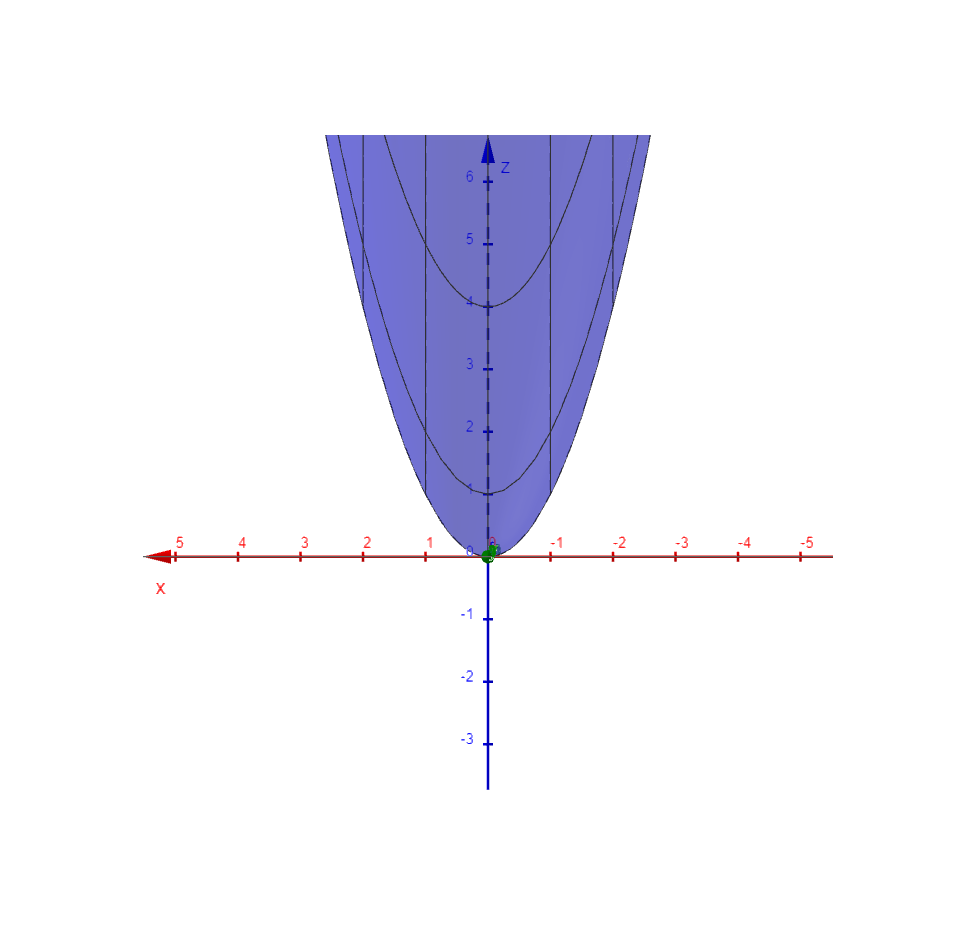
\includegraphics[width=\textwidth]{Capitoli/Capitolo2/Minimo.png}
            \caption{Grafico di $f(x,y)=x^2+y^2$ che mostra un minimo in $(0,0)$.}
        \end{minipage}
        \hspace{1cm}
        \begin{minipage}{0.26\textwidth}
            \centering
            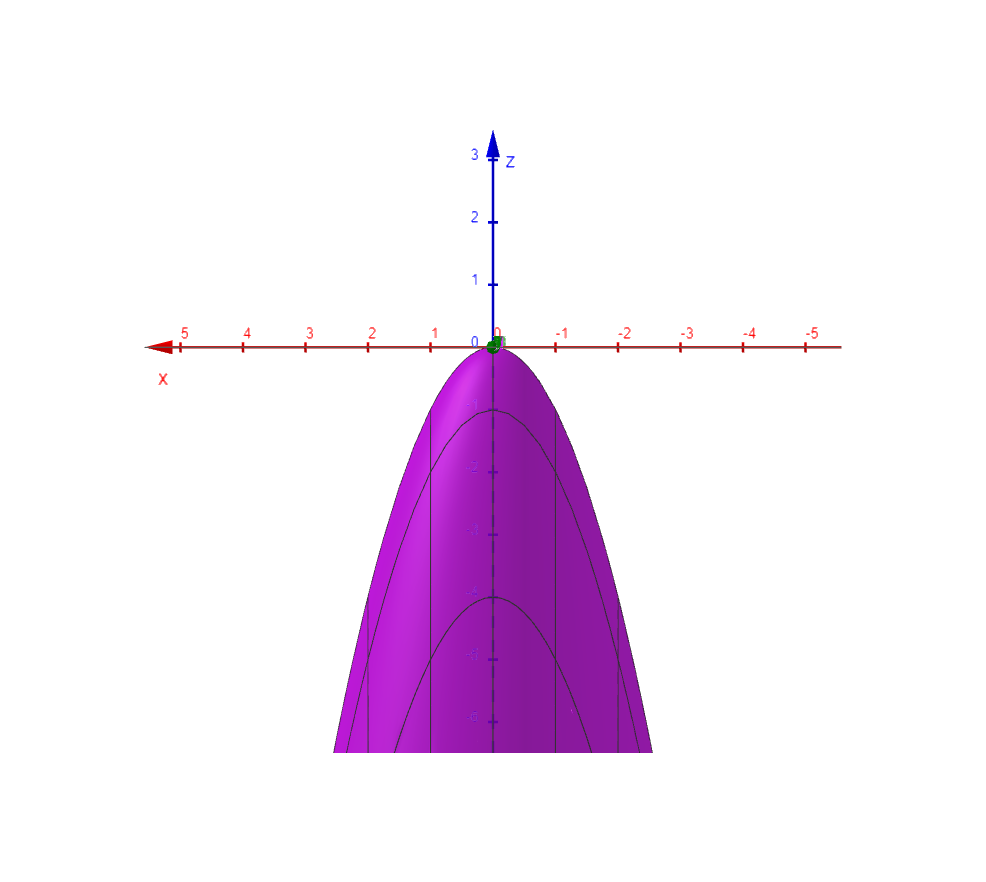
\includegraphics[width=\textwidth]{Capitoli/Capitolo2/Massimo.png}
            \caption{Grafico di $f(x,y)=-x^2-y^2$ che mostra un massimo in $(0,0)$.}
        \end{minipage}
        \hspace{1cm}
        \begin{minipage}{0.26\textwidth}
            \centering
            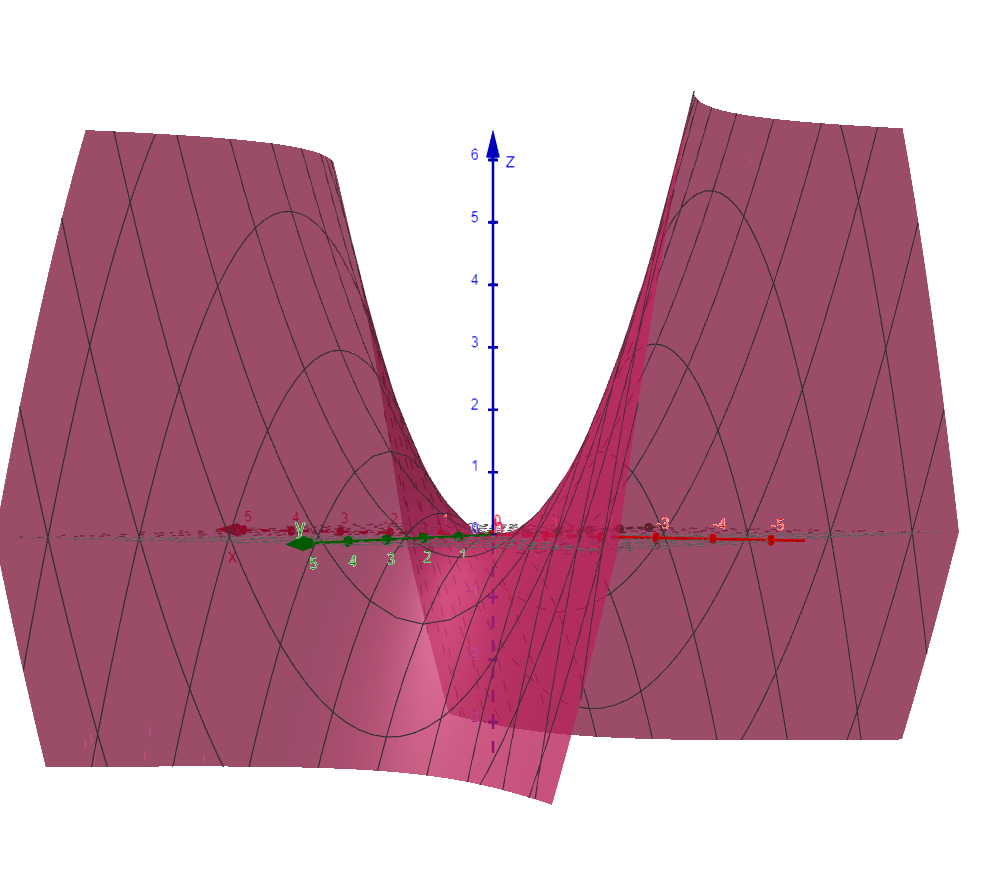
\includegraphics[width=\textwidth]{Capitoli/Capitolo2/Sella 3.png}
            \caption{Grafico di $f(x,y)=\frac{x^2}{3}-\frac{y^2}{3}$ che mostra punto di sella in $(0,0)$.}
        \end{minipage}
    \end{figure}
\end{example}
\paragraph{Richiami sulle forme quadratiche} Una \textbf{forma quadratica} è un polinomio omogeneo di secondo grado tale che
\begin{equation}
    q(\lambda x)=\lambda^2 q(x)\ \forall x \in \mathbb{R}^n,\ \lambda \in \mathbb{R}
\end{equation}
In particolare ad una forma quadratica può essere associata univocamente una matrice rappresentativa simmetrica definita come 
\begin{equation}
    Q=q_{ij}\ \text{con}\ q_{ij}=\frac{a_{ij}+a_{ji}}{2}
\end{equation}
tale che
\begin{equation}
    q(x)=\langle Qx, x \rangle
\end{equation}
\begin{oss}
    Si può notare come nel teorema di Taylor la forma $\langle H_f(x_0)h, h \rangle$ sia una forma quadratica \textit{indotta} da $H_f$.
\end{oss}
Inoltre, una forma quadratica può essere detta:
\begin{itemize}
    \item \textit{Definita positiva (negativa)} se $\forall\ \lambda_i$ si ha che $\lambda_i \underset{(<)}{>}0$
    \item \textit{Semidefinita positiva (negativa)} se $\forall\ \lambda_i$ si ha che $\lambda_i \underset{(\leq)}{\geq}0$
    \item \textit{Indefinita} se $\exists\ \lambda_i, \lambda_j$ tali che $\lambda_i\lambda_j<0$
\end{itemize}
\paragraph{Classificazione dei punti critici} Sia $x_0 \in A$ un punto critico per $f:A \subseteq \mathbb{R}^n\to \mathbb{R}$. Allora il polinomio di Taylor con resto di Peano al secondo ordine è
\begin{equation}
    \begin{aligned}
        f(x_0+h)&=f(x_0)+ \langle \nabla f(x_0), h\rangle+ \frac{1}{2}\langle H_f(x_0)h,h \rangle +o(|h|^2)=\\ 
        &= f(x_0)+ \frac{1}{2}\langle H_f(x_0)h,h \rangle + o(|h|^2)
    \end{aligned}
\end{equation} 
Quindi, per poter fornire dei criteri di classificazione dei punti critici occorre studiare il segno della forma quadratica indotta da $H_f$.
\begin{proposition}
    Sia $f:A \subseteq \mathbb{R}^n \to \mathbb{R}$ e sia $f \in C^2(A)$. Sia poi $x_0$ un punto critico per $f$.\\
    Se $x_0$ è un massimo relativo, allora $H_f(x_0)$ è (semi)definita negativa.
    \begin{equation}
        \langle H_f(x_0)h, h \rangle \underset{(\leq)}{<} 0
    \end{equation}
    Se $x_0$ è un minimo relativo, allora $H_f(x_0)$ è (semi)definita positiva.
    \begin{equation}
        \langle H_f(x_0)h, h \rangle \underset{(\geq)}{>} 0
    \end{equation}
\end{proposition}
\begin{theorem} [Condizione necessaria del II ordine] \label{Teo: Condizione necessaria del secondo ordine}
Sia $f: A \subseteq \mathbb{R}^n \to \mathbb{R}$ e sia $x_0 \in A$ critico per $f$. Sia poi $f \in C^2(A)$. Se $x_0$ è massimo (minimo) relativo, allora $H_f(x_0)$ è semidefinita negativa (positiva).
\end{theorem}
\begin{proof}
    Sia $x_0$ un punto di massimo relativo per $f$ , sia $v \in \mathbb{R}^n$ direzione fissata. Si definisca allora
    \begin{equation}
    F(t)=f(x_0+tv)
    \end{equation}
    Siccome $A$ è aperto, $F$ è definita su un certo $\left(-\delta, \delta\right)$ con $\delta>0$. Per ipotesi su $f$, $F$ ha un massimo relativo in $t=0$ ed è di classe $C^2(-\delta, +\delta)$.\\
    Per l'equazione \eqref{Eq: Premessa al teo Lagrange}, si ottiene che
    \begin{equation}
        F''(t)= \langle H_f(x_0+tv)v, v \rangle 
    \end{equation}
    da cui, per condizione necessaria sulle funzioni di una variabile, segue che
    \begin{equation}
        F''(0)= \langle H_f(x_0)v, v \rangle \leq 0
    \end{equation}
    cioè che $H_f(x_0)$ è semidefinita negativa.\\
    La dimostrazione del caso in cui $x_0$ è minimo relativo per $f$ è del tutto analoga.
\end{proof}
\begin{lemma} \label{Lemma: FQ di matrice simmetrica è compresa tra i suoi autovalori max e min}
        Se, presa $A \in \mathbb{M}_{n,n}$ simmetrica e detti $\lambda_1 \leq \lambda_2 \leq \lambda_n$ i suoi autovalori, si ha $\langle Ax, x \rangle$, allora $\lambda_1 |x|^2 \leq \langle Ax, x \rangle \leq \lambda_n |x|^2$
\end{lemma}
\begin{theorem}[Condizione sufficiente del II ordine] \label{Teo: Condizione sufficiente del secondo ordine}
    Sia $f:A \subseteq \mathbb{R}^n \to \mathbb{R}$ e sia $f \in C^2(A)$. Sia poi $x_0$ un punto critico per $f$. Allora, 
    \begin{itemize}
        \item Se $H_f(x_0)$ è definita positiva (negativa), allora $x_0$ è un minimo (massimo) relativo.
        \item Se $H_f(x_0)$ è indefinita, allora $x_0$ è un punto di sella.
    \end{itemize}
\end{theorem}
    \begin{proof}
        Si consideri il caso in cui $H_f(x_0)$ sia definita positiva e si mostri che $x_0$ è un punto di minimo per $f$\\
        Si può osservare che, essendo $f \in C^2(A)$, allora $H_f$ è simmetrica per il teorema \ref{Teo: Schwarz} e vale dunque il lemma \ref{Lemma: FQ di matrice simmetrica è compresa tra i suoi autovalori max e min}. Pertanto, indicato con $\lambda_{min}>0$ il minor autovalore di $H_f$, si ha che
        \begin{equation}
            \langle H_f(x_0)h,h \rangle \geq \lambda_{min} |h|^2 \qquad \forall h \in \mathbb{R}^n
        \end{equation}
        Si scriva quindi lo sviluppo di Taylor con resto di Peano al secondo ordine in $f(x_0)$.
        \begin{equation}
        \begin{aligned}
            f(x_0+h)-f(x_0)&= \langle \nabla f(x_0), h \rangle + \frac{1}{2}\langle H_f(x_0h, h\rangle + o(|h|^2)=\\
            &\overset{f'(x_0)=0}{=} \frac{1}{2}\langle H_f(x_0)h, h\rangle + o(|h|^2) \geq \\
            &\overset{\text{Lemma}\ \ref{Lemma: FQ di matrice simmetrica è compresa tra i suoi autovalori max e min}}{\geq} \frac{1}{2} \lambda_{min}|h|^2+o(|h|^2)
        \end{aligned}
        \end{equation}
        Poiché scopo della dimostrazione è mostrare che $f(x_0+h)-f(x_0) \geq 0\ \forall h \in \mathbb{R}^n$, occorre provare che $o(|h|^2)$ sia trascurabile.
        \begin{equation}
            f(x_0+h)- f(x_0) \geq \frac{1}{2}\lambda_{min} |h|^2 \left( 1 + \frac{o(|h|^2)}{\tfrac{1}{2}\lambda_{min}|h|^2}\right)
        \end{equation}
        ma, per definizione di o-piccolo vale il seguente fatto:
        \begin{equation}
            \exists\ \sigma >0\ \text{tale che, se}\ |h|<\sigma\ \text{allora}\ \left|\frac{o(|h|^2)}{\tfrac{1}{2}\lambda_{min} |h|^2}\right| < \frac{1}{2}
        \end{equation}
        dove $\sigma=\frac{1}{2}$ è una costante arbitraria in $(0,1)$.
        Per tale disuguaglianza, allora, 
        \begin{equation}
        \begin{aligned}
            f(x_0+h)-f(x_0)&\geq \frac{1}{2}\lambda_{min} |h|^2 \left( 1 + \frac{o(|h|^2)}{\tfrac{1}{2}\lambda_{min}|h|^2}\right) \geq \\
            &\geq \frac{1}{2}\lambda_{min}|h|^2\left(1-\frac{1}{2}\right)=\frac{1}{4}\lambda_{min}|h|^2 >0
            \end{aligned}
        \end{equation}
        purché $|h|< \sigma$. In tal caso la definizione di minimo è soddisfatta.\\
        La dimostrazione per $H_f(x_0)$ definita negativa è analoga.\\
    Si dimostri ora il punto 2.\\
    Se $H_f(x_0)$ è indefinita, allora non soddisfa le ipotesi della condizione necessaria del secondo ordine (teorema \ref{Teo: Condizione necessaria del secondo ordine}), cioè non è né massimo né minimo. Quindi, essendo per ipotesi critico, deve essere una sella.
    \end{proof}
    \begin{oss}
        Se vale $f(x_0+h)-f(x_0) \gtrless 0$, $x_0$ si dice minimo (massimo) forte.
    \end{oss}
    \begin{oss}
        Si noti che non è possibile concludere niente previa indagine nel caso in cui $H_f$ sia semidefinita.
    \end{oss}
    \paragraph{Metodo delle restrizioni} Come accennato, se $H_f(x_0)$ è semidefinita, non è possibile caratterizzare il punto critico. Si mostri allora un metodo per farlo tramite esempio.
    \begin{example}
        Sia $f(x,y)=x^4-y^4$. Allora il punto $(0,0)$ è critico e si ha che
        \begin{equation*}
            H_f(0,0)=\begin{pmatrix}
                0 & 0\\
                0 & 0
            \end{pmatrix}
        \end{equation*}
        con $f(0,0)=0$. Si può osservare, però che:
        \begin{equation*}
            \begin{aligned}
                &f(x, 0) > 0 \qquad \forall x \neq 0\\
                &f(0,y) < 0 \qquad \forall y \neq 0
            \end{aligned}
        \end{equation*}
        Pertanto $(0,0)$ è un punto di sella, giacché non è né un massimo né un minimo.
    \end{example}
    Può capitare, però, di non trovare restrizioni di quel genere, allora bisogna ricorrere allo studio del segno di
    \begin{equation*}
        f(x)-f(x_0)
    \end{equation*}
\section{Funzioni a valori vettoriali}
\begin{definition} \label{Def: Funzioni a valori vettoriali}
    Siano $n,\ m \in \mathbb{N}$ e sia $A \subseteq \mathbb{R}^n$. Allora si dice che una funzione $f$ è \textbf{a valori vettoriali} se è così definita:
    \begin{equation}
    \begin{aligned}
        f:A \subseteq \mathbb{R}^n &\to \mathbb{R}^m\\
        (x_1, \dots, x_n) &\mapsto (f_1(x_1, \dots, x_n), \dots, f_n(x_1, \dots, x_n))
    \end{aligned}
    \end{equation}
\end{definition}
\begin{oss}
    Si noti che limiti, continuità e derivabilità vanno estese ad un ragionamento componente per componente.
\end{oss}
\begin{oss}
    Se la dimensione del dominio e del codominio è la medesima, si parla di \textit{campo vettoriale}.
\end{oss}
\begin{definition} \label{Def: Derivabilità di f. vettoriali}
    Si dice che $f:A \subseteq \mathbb{R}^n \to \mathbb{R}^m$ è \textbf{derivabile} in $x_0 \in A$ se ciascuna $f_i$ con $i=1, \dots, n$ è ivi derivabile.
\end{definition}
\begin{definition} \label{Def: Matrice Jacobiana}
    Se $f$ è derivabile in $x_0$, si dice \textbf{matrice jacobiana} di $f$ in $x_0$ la matrice $J_f \in \mathbb{M}_{m,n}$ definita da
    \begin{equation} \label{Eq: Matrice Jacobiana}
        J_f(x_0)=\begin{pmatrix}
            \frac{\partial{f_1}}{\partial{x_1}}(x_0) & \frac{\partial{f_1}}{\partial{x_2}}(x_0)& \dots & \frac{\partial{f_1}}{\partial{x_n}}(x_0)\\
            \frac{\partial{f_2}}{\partial{x_1}}(x_0)& \frac{\partial{f_2}}{\partial{x_2}}(x_0)& \dots & \frac{\partial{f_2}}{\partial{x_n}}(x_0)\\
            \vdots & \vdots & \ddots & \vdots\\
            \frac{\partial{f_n}}{\partial{x_1}}(x_0) & \frac{\partial{f_n}}{x_2}(x_0)& \dots & \frac{\partial{f_n}}{\partial{x_n}}(x_0)
        \end{pmatrix}
        =
        \begin{pmatrix}
            \nabla f_1 (x_0)\\
            \nabla f_2(x_0)\\
            \vdots\\
            \nabla f_n(x_0)
        \end{pmatrix}
    \end{equation}
    Il determinante della matrice Jacobiana è detto \textbf{Jacobiano} \label{Def: Jacobiano}
\end{definition}
\begin{definition} \label{Def: Differenziabilità di f. vettoriali}
    Una funzione $f$ si dice \textbf{differenziabile} in $x_0 \in A$ se
    \begin{equation}
        \lim_{h \to 0}{\frac{f(x_0+h)-f(x_0)-J_f(x_0)h}{|h|}}=0
    \end{equation}
\end{definition}

\begin{theorem} \label{Teo: Derivata composta di f. vettoriali}
Siano $g: B \subseteq \mathbb{R}^k \to A \subseteq R^n$ e $f: A \subseteq \mathbb{R}^n \to \mathbb{R}^m$ e le si assuma di classe $C^1$. Allora, $h=f \circ g: B \to \mathbb{R}^m$ è ben definita su $B$, è di classe $C^1(B)$ e vale:
\begin{equation}
    J_h(y) \in \mathbb{M}_{m,n}\ \text{tale che}\ J_h(y)=J_f(g(y)) J_g(y) \qquad \forall\ y \in B
\end{equation}
\end{theorem}
\begin{oss}
    Essendo di classe $C^1$, $h$ è differenziabile, in accordo con i ragionamenti già svolti nell'equazione \eqref{Eq: Relazione C^1 -> diff -> C^0}.
\end{oss}